\documentclass[12pt]{article}

\usepackage[margin=50pt]{geometry}
\usepackage{amsmath}
\usepackage{amssymb}
\usepackage{graphicx}
\usepackage{algorithm}
\usepackage{algpseudocode}
\usepackage{subcaption}

\DeclareMathOperator*{\argmax}{argmax}
\DeclareMathOperator*{\argmin}{argmin}

\graphicspath{/images}
\geometry{footskip=0.8cm}

\title{Intelligent Systems}
\author{Thomas Vroom}

\begin{document}
\maketitle

%
% Topic 1 - (Artificial) Intelligence
%
\section{(Artificial) Intelligence}
The everyday notion of intelligence is used as the starting point of artificial intelligence (AI).
An indirect goal of artificial intelligence research is to achieve the computational precision of this everyday notion.
This resulted in a multidisciplinary field dealing with the design, analysis and application of computer-based systems that deserve to be called \textit{intelligent}.

\noindent
\\
A problem for the research field of artificial intelligence is that there is no commonly accepted definition of intelligence.
It is generally believed that intelligent systems must be \textbf{capable} (be able to do something), \textbf{autonomous} (operate without human intervention) and \textbf{believable} (convince humans it is intelligent), but this is not an official definition.

\subsection{The Turing Test}
The Turing test (originally known as \textit{the imitation game}) was proposed by Alan Turing in 1950 as a "killer test" for artificial intelligence.
The idea is that a computer system is intelligent if it can answer some questions by a person in such a way that this person cannot tell if the answers are given by a human or a computer.

\noindent
\\
This is an operational definition of intelligence, since it is defined on the basis of indistinguishability from human intelligence.
It is also related to the \textbf{Theory of Mind}, which is the ability of humans to image the mental states of others.

\noindent
\\
With the recent advances in AI, we are already at the point where we can create systems that can trivially pass the Turing test (some examples are ChatGPT and Google Duplex).

\subsection{Supercriticality}
Turing also proposed the concept of a \textbf{subcritical} and a \textbf{supercritical} brain.
A hot topic at the time was the notion of subcritical or supercritical mass, when trying to create a nuclear reaction.
Instead of injecting neutrons into a mass of uranium, Turing made the analogy of injecting ideas into a brain.

\noindent
\\
When putting an idea into a subcritical brain, it will on average return less than 1 new idea.
This is the case for human brains, since we forget most thoughts we have.
But when putting an idea into a supercritical brain, it will on average return more than 1 new idea.
Ongoing research is still trying to figure out if it is possible to create an (artificial) supercritical brain.

\newpage
\noindent
In one of his last papers before his dead, computer scientist John McCarthy stated that machine learning only finds relations between observations, which means it is not capable of discovering new knowledge.
If all you ever knew was that you have to swim across a river to get to the other side, you would never discover the concept of a bridge.
This resembles a subcritical brain that will never return more than is given.

\noindent
\\
Arguments against McCarthy's statement mainly focus on the idea of \textbf{abductive reasoning} (seeking the simplest and most likely explanation for a set of observations), as well as \textbf{latent space embedding} (transforming observations into an explorable space).

\subsection{The Chinese Room Thought Experiment}
Current motivations for AI research are often either \textbf{visionary} (the belief that AI will be able to \textit{produce} intelligent behavior), or \textbf{pragmatic} (the belief that AI will be able to \textit{simulate} intelligent behavior).
This has lead to the debate on \textbf{Strong AI} vs. \textbf{Weak AI}.
Intelligent systems that are capable of thinking and understanding are referred to as strong AI, while systems that are only pretending to be intelligent are referred to as weak AI.

\noindent
\\
A common way to think about the difference between strong AI and weak AI is the \textbf{Chinese Room Thought Experiment}: Does a person locked in a room with a rule book and a set of Chinese symbols, answering questions in Chinese, understand Chinese?
Does ChatGPT understand the answers it gives to your questions?

\begin{figure}[h]
    \centering
    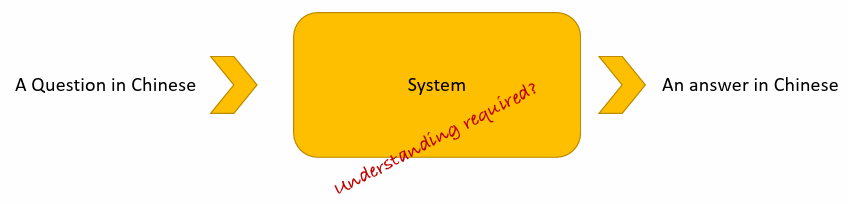
\includegraphics[scale=0.8]{images/chineseroom.PNG}
\end{figure}
\vspace{-0.5cm}

\subsection{Historical Concepts}
Throughout the years, many concepts of artificial intelligence have been proposed.
Since then the field has obviously evolved, but just because a concept is old does not mean it is irrelevant.

\subsubsection{Knowledge-Based AI}
In the field of knowledge-based AI, it is thought that AI is all about being able to \textit{think}.
Therefore, the guiding model of this field is the individual human reasoning capabilities.
An important assumption in this field is that intelligence is a combination of knowledge representation and processing, for which a Von Neumann computer is the best model of the human "cognitive apparat".

\noindent
\\
Knowledge-based AI works with the \textbf{symbol system hypothesis}, stating that being able to produce and manipulate \textbf{symbols} (a representation of something) is a necessary and sufficient condition for intelligence.
A major problem with this is \textbf{symbol grounding}, which means how to relate symbols to the real world.

\newpage
\subsubsection{Behavior-Based AI}
Behavior-based AI is based on the idea that intelligence can emerge from the interaction of simple behaviors.
A common example used to explain this is an ant colony, where the individual ants are not seen as intelligent, but the colony as a whole is.

\noindent
\\
An important hypothesis in this field is the \textbf{physical grounding hypothesis}, stating that symbols must be grounded in the real world (in which the agents act), and that this is a necessary condition for intelligence.
It is believed that if symbols are not grounded, that they do not carry any meaning and are therefore irrelevant for "intelligent behavior".

\noindent
\\
A big difference between knowledge-based AI and behavior-based AI is how they are constructed.
Knowledge-based AI is often constructed with a \textbf{top-down} design, where you start with high level concepts and slowly break them down into smaller, programmable units.
Behavior-based AI is often constructed with a \textbf{bottom-up} design, where you start with simple behaviors and slowly build them up into more complex behaviors.

\subsubsection{Connectionism}
The guiding assumption of connectionism is that intelligence can be simulated by processing information through simple, but many interconnected units (neurons) that interact at a low level.
The idea is that if you combine enough of these simple processing units, you can do some pretty complex operations.
A common architecture used in connectionism is \textbf{artificial neural networks}, originally modeled after the human brain.
The key characteristics of connectionism are \textbf{parallelism} and \textbf{sub-symbolic information processing}.

\subsubsection{Distributed AI}
The main idea behind distributed AI is that intelligence cannot be simulated through a single 'box'.
The guiding assumptions of this field are that interacting together is a characteristic of intelligent beings, and that there is no intelligence without interaction.
In contrast to connectionism, in distributed AI the interacting units interact on the \textbf{knowledge level}, rather than the \textbf{signal level}.

\noindent
\\
The key characteristics of distributed AI are \textbf{parallelism}, \textbf{scalability} and \textbf{robustness} (stepping on a single ant does not destroy the whole colony).
A common belief is that some problems can \textit{only} be solved through high level interaction among intelligent agents, similar to how humans cooperate.

%
% Topic 2 - Agent Concepts
%
\newpage
\section{Agent Concepts}
Similarly to intelligence, there is no commonly accepted definition of an agent either.
An emerging standard view in the field of AI however, is that an agent is a (computational) entity that is \textbf{situated} in some environment, and is capable of \textbf{flexible}, \textbf{autonomous} activity in order to meet its design objectives.
Other characteristics that are sometimes claimed to be essential include:

\begin{itemize}
    \item \textbf{Rationality:} making logical decisions based on the circumstances.
    \item \textbf{Mobility:} being able to move around in the environment.
    \item \textbf{Introspection:} think about what it is doing and why it is doing it.
    \item \textbf{Benevolence:} being well-meaning and not causing harm.
\end{itemize}

\noindent
Agents, in programming terms, are often confused with objects.
Both encapsulate identity (who), state (what) and passive behavior (how), but agents additionally encapsulate \textbf{active behavior:} when, why, with whom and whether at all.

\noindent
\\
A \textbf{minimally intelligent agent} is known as the bare minimum of what we need to call an agent "intelligent".
The requirements for a minimally intelligent agent are:

\begin{itemize}
    \item \textbf{Pro-activeness:} the ability to take initiative.
    \item \textbf{Reactivity:} the ability to perceive and (timely) respond to the environment.
    \item \textbf{Social ability:} the ability to interact with humans and other agents.
\end{itemize}

\noindent
Functional systems that are externally activated (e.g. sending out an email) are called \textbf{goal-directed systems}.
While systems that constantly need to adapt to a changing environment (e.g. flying a plane) are called \textbf{reactive systems}.
The great difficulty in creating intelligent agents is balancing goal-directedness with reactivity.
Such a hybrid agent must be able to react to a new, unseen situation while also focussing on getting things done.

\subsection{Agent Environment}
An agent is always situated in an environment, which is the context in which the agent operates.
An environment can be described by the following characteristics:

\begin{itemize}
    \item \textbf{Accessible vs. Inaccessible:} the level of information the agent gets about its environment (complete? acurate? up-to-date?)
    \item \textbf{Deterministic vs. Non-deterministic:} is there a guaranteed effect for actions? is there uncertainty about the next state? Note that sufficiently complex determinism is just as bad as non-determinism.
    \item \textbf{Episodic vs. Non-episodic:} if there are independent stages of behavior (i.e. future is independent of past).
    \item \textbf{Static vs. Dynamic:} if the actions of the agent are the only cause for change in the environment.
    \item \textbf{Discrete vs. Continuous:} if the environment is made up of a finite number of states and actions.
\end{itemize}

\newpage
\subsection{Agent Architectures}
\subsubsection{Logic Based Agents}
Logic based agents are build on the idea of knowledge based AI.
The idea is that intelligent behavior is a result of a symbolic representation of the environment combined with logical deduction or theorem proving:
\[ \Delta \vdash_\rho \varphi \]

\noindent
Here $\varphi$ represents the action chosen by the agent, $\Delta$ represents the \textbf{belief database:} all information the agent has about the environment, and $\rho$ represents the \textbf{theory of agency:} a description of how the agent behaves in an executable way.
A common example used with logic based agents is a vacuum agent:

\begin{figure}[h]
    \centering
    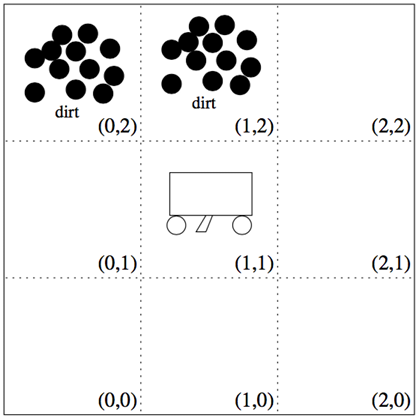
\includegraphics[scale=0.6]{images/vacuumagent.PNG}
\end{figure}

\noindent
This world can be described using the following symbols:

\begin{itemize}
    \item $In(x, y) :=$ agent is at $(x, y)$.
    \item $Dirt(x, y) :=$ there is dirt at $(x, y)$.
    \item $Facing(d) :=$ the agent is facing in direction $d$.
\end{itemize}

\noindent
\textbf{Action rules} for logic based agents are defined in the form of "if you can prove this, then do this":
\[ \varphi(...) \longrightarrow \psi(...) \]

\noindent
For the vacuum agent, an example action rule would be:
\[ In(x, y) \wedge Dirt(x, y) \longrightarrow Do(suck) \]

\noindent
Logic based agents have a few problems:

\begin{itemize}
    \item \textbf{Symbol grounding:} how to relate symbols to the real world.
    \item \textbf{Temporal information:} how to deal with time (e.g. how long to suck up all the dirt?).
    \item \textbf{Complex environments:} building a sufficiently complete model takes a lot of time.
\end{itemize}

\noindent
However, this does not mean logic based agents are irrelevant.
Logic based agents start to shine when combined with learning algorithms (e.g. deep learning, reinforcement learning), which help overcome the problems mentioned above.

\newpage
\subsubsection{Simple Reactive Agents}
The main idea behind simple reactive agents is that intelligence emerges from the interaction between \textbf{simple} behaviors and \textbf{direct} observations of the environment.
The architecture of a simple reactive agent looks like this:

\begin{figure}[h]
    \centering
    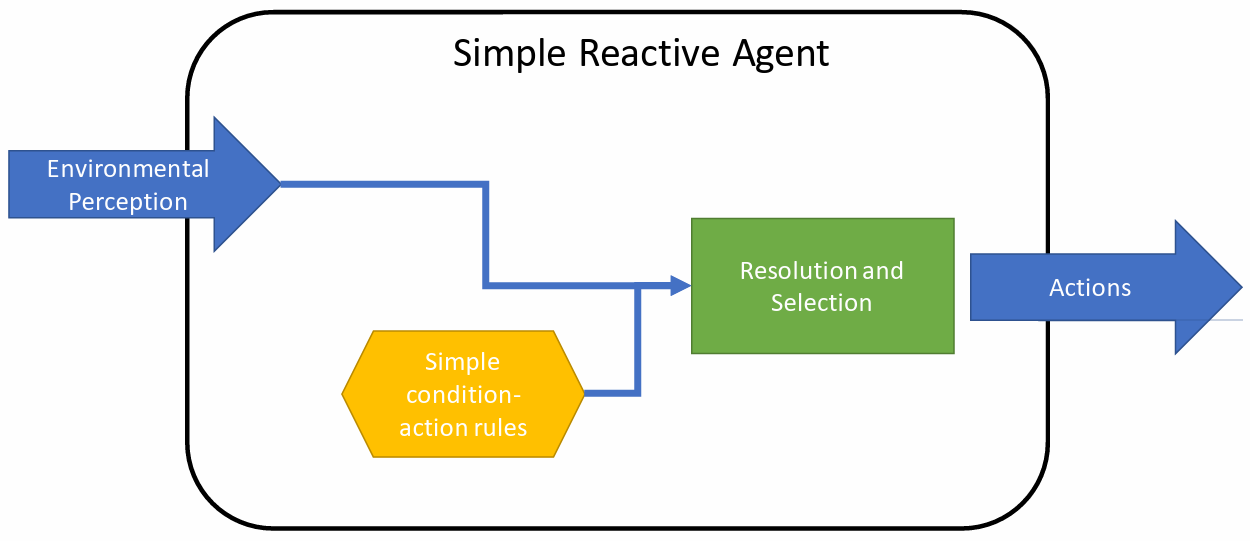
\includegraphics[scale=0.5]{images/simplereactiveagent.PNG}
\end{figure}

\noindent
The decision-making of these agents is established through a set of behaviors.
Each behavior accomplishes some sort of subtask.
There is no complex symbolic reasoning going on, just a direct mapping from observations to actions.
When multiple behaviors choose conflicting actions, the agent refers to the \textbf{subsumption hierarchy}.

\noindent
\\
Advantages of simple reactive agents is that they are simple, fast and robust against failure.
However, the also have a set of drawbacks.
These include the fact that only local information is used (there is no model of the environment), the short term view of the agent, the fact that emergence can be hard to predict, and the fact that the dynamics of interactions can become too complex.

\subsubsection{Model-based Reactive Agents}
If the environment is assumed to be Markovian, then we can use reinforcement learning to create a reactive agent that learns a reactive policy.
If the environment is not Markovian, then the agent maintains a set of beliefs about the state of the environment.
The architecture of a model-based reactive agent looks like this:

\begin{figure}[h]
    \centering
    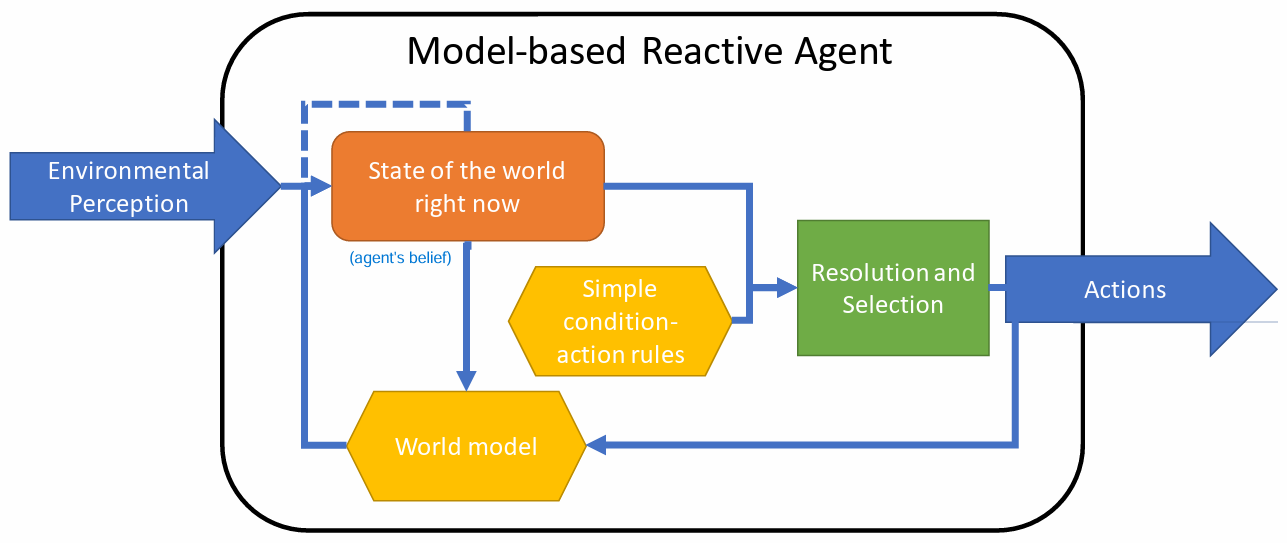
\includegraphics[scale=0.5]{images/modelbasedreactiveagent.PNG}
\end{figure}

\newpage
\subsubsection{Goal-based Agents}
A problem with the previous architectures is that they are not capable of changing their goal state depending on the environment, whilst this is a key characteristic of intelligent behavior.
We can therefore extend the model-based reactive agent to a goal-based agent:

\begin{figure}[h]
    \centering
    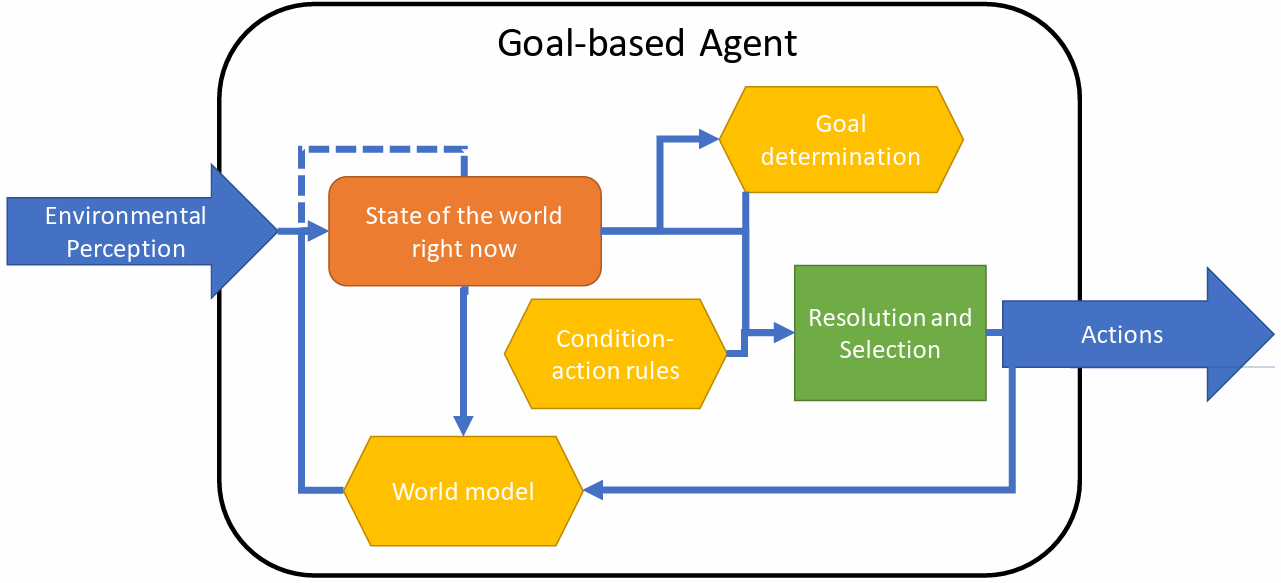
\includegraphics[scale=0.5]{images/goalbasedagent.PNG}
\end{figure}

\noindent
There are two types of strategies for goal-based agents:

\begin{itemize}
    \item \textbf{Bold agents:} agents that never stop to reconsider their goals.
    \item \textbf{Cautious agents:} agents that constantly stop to reconsider their goals.
\end{itemize}

\noindent
This leads to a new problem: how to balance goal-directedness with reactivity?

\begin{figure}[h]
    \centering
    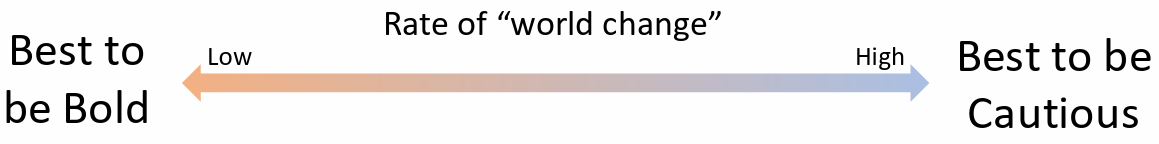
\includegraphics[scale=0.5]{images/boldvscautious.PNG}
\end{figure}

\noindent
This problem can be solved using \textbf{Layered Architectures}.

\subsection{Layered Architectures}
Layered architectures are needed for both proactive (i.e. reach the goal) and reactive (i.e. reconsider) behavior.
This naturally leads to multiple interacting layers of hierarchically organized behaviors.

\subsubsection{Horizontal Layering}
In a horizontal layered architecture, the number of layers is equal to the number of desired behaviors.
Similarly to simple reactive agents, we might need a mediator function if multiple behaviors conflict, but this central control might create bottlenecks if the number of behaviors is large.

\newpage
\begin{figure}[h]
    \centering
    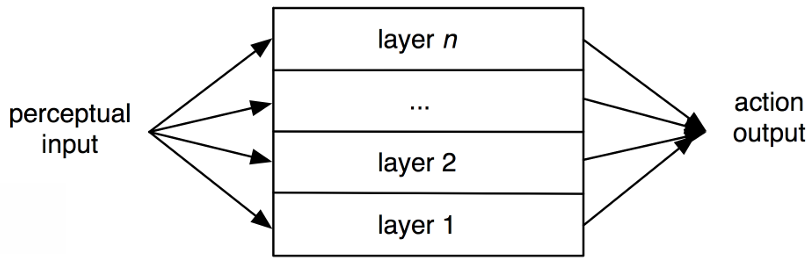
\includegraphics[scale=0.5]{images/horizontallayering.PNG}
\end{figure}

\subsubsection{Vertical Layering}
\begin{figure}[h]
    \centering
    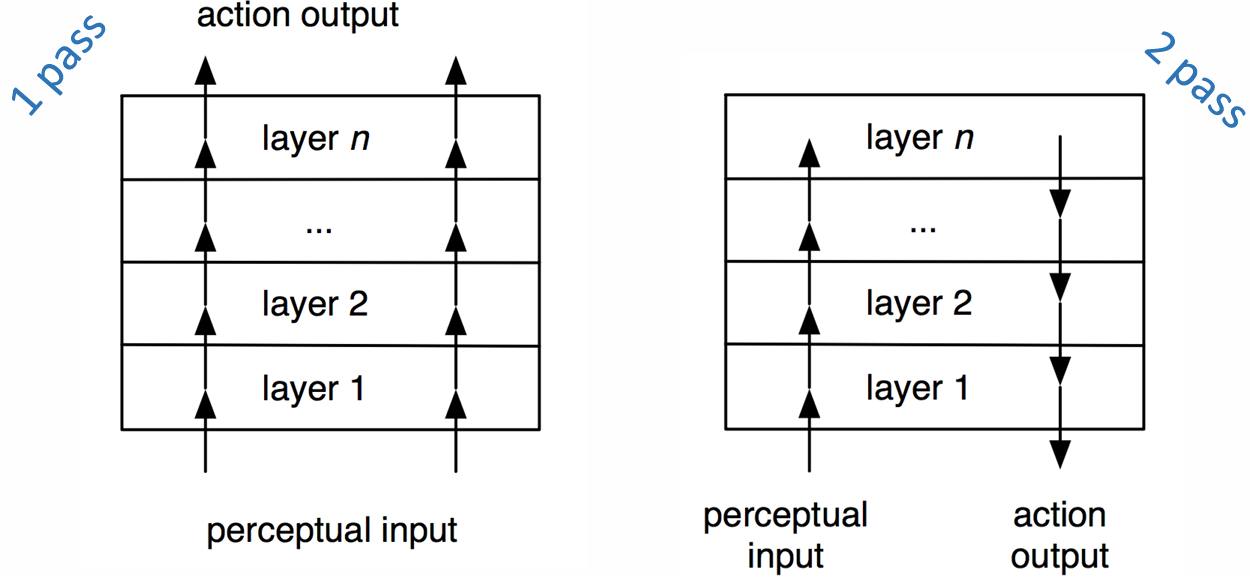
\includegraphics[scale=0.5]{images/verticallayering.PNG}
\end{figure}

\noindent
Vertical layered architectures build upon layers of abstraction to create more complex behaviors.
These architectures are often used in the field of robotics, where the layers are referred to as sense-plan-act.
2-pass vertical layered architectures are first activated \textbf{bottom-up}, then executed \textbf{top-down}.

%
% Topic 3 - Expert Systems
%
\newpage
\section{Expert Systems}
An expert system is a computer system that emulates the decision-making ability of a human expert.
In more detail, an expert system is a computer system that uses \textbf{knowledge} and \textbf{inference} to solve problems in a \textbf{specialized subject domain}, that are difficult enough to require \textbf{human expertise}.

\noindent
\\
Expert systems are not traditionally seen as "intelligent systems": they are not proactive or autonomous, and have no real world embedding.
Expert systems are often compared to \textbf{decision support systems (DSS)}, which are systems that help humans make decisions, rather than making decisions themselves.
The main difference between the two is that expert systems are capable of providing recommendations (often as the last step), while decision support systems will only provide information.

\noindent
\\
Expert systems are often used as a \textbf{diagnosis tool}, for example in the medical field or in the field of maintenance.
A common example of an expert system is the software that a car mechanic plugs into your car when it comes to the garage.
The reason for its popularity is that expert systems are \textbf{provably correct}.
In some industries this is a very important characteristic, for example when sending a rover to Mars.

\subsection{Components of an Expert System}
An expert system consists of the following components:

\begin{figure}[h]
    \centering
    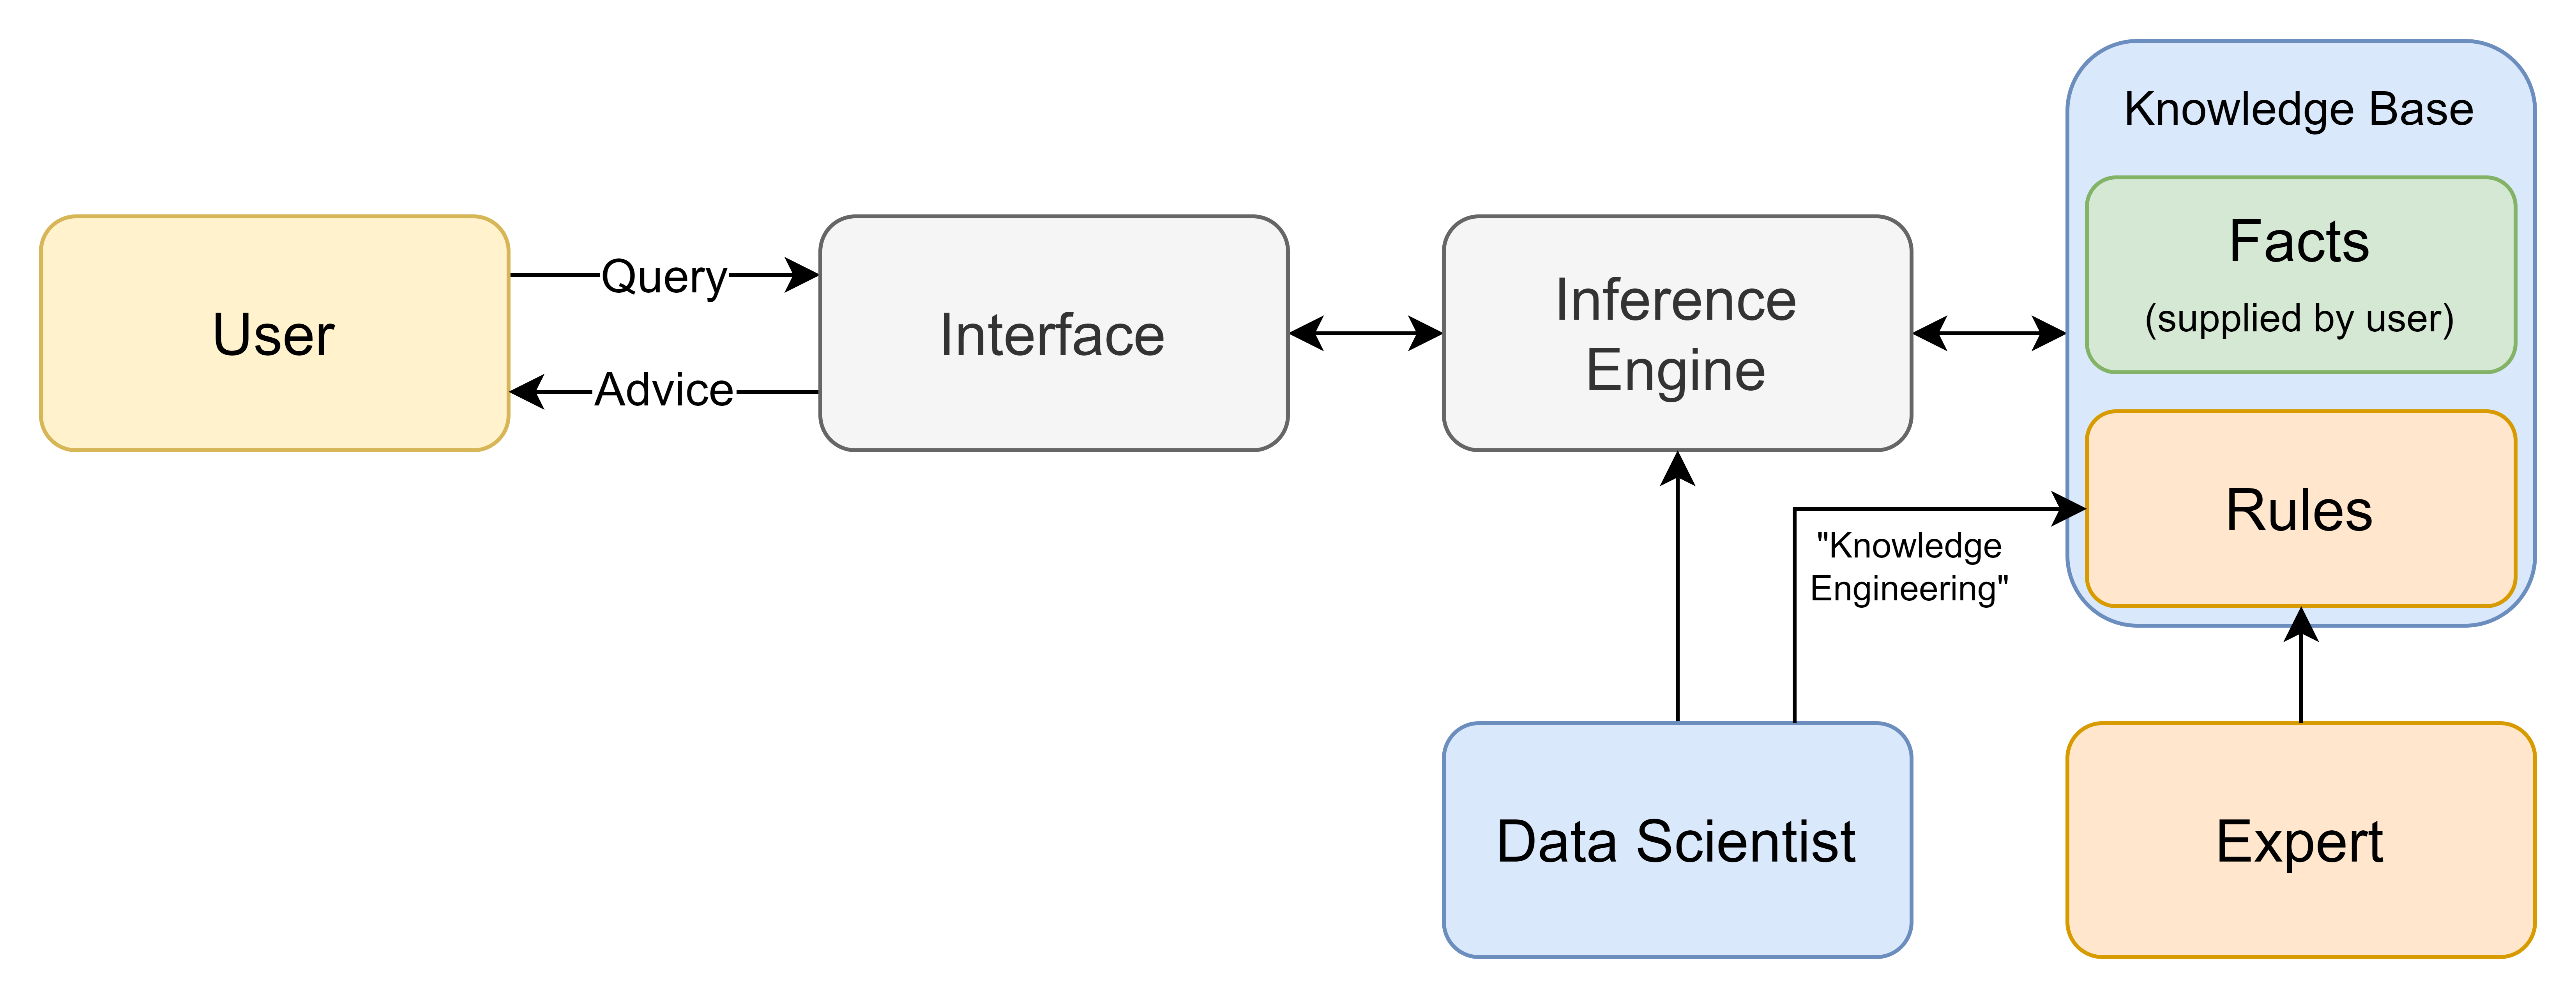
\includegraphics[scale=0.075]{images/expertsystemdiagram.png}
\end{figure}

\noindent
The user interacts with the interface to provide the expert system with information, along with a query about the problem.
The expert system uses an \textbf{inference engine} to reason about the problem, together with the information provided by the user and a predefined set of rules provided by experts.
The process of generating these rules from experts is called \textbf{knowledge engineering}.
Once the expert system has reached a conclusion, it will provide the user with an appropriate advice, along with an explanation of how it constructed this advice.

\noindent
\\
The inference engine and expert rules must be defined using the same \textbf{knowledge representation}.
Examples of commonly used knowledge representations are first order logic, ontologies and non-monotonic logics (logics that allow for exceptions).

\newpage
\subsection{Probabilistic Reasoning}
A difficult problem in expert systems is how to incorporate uncertainty into the model.
Uncertainty is often given in the form of \textbf{probabilistic facts}, for example:
\[ P(\text{rain tomorrow}) = 0.6 \]
\[ P(\text{heads}) = 0.5 \]

\subsubsection{Marginalization and Maximization}
\textbf{Marginalizing} means finding the probability of a certain variable, or collection of variables:
\[ P(X_1 = p_1) \text{ or } P(X_1 = p_1, X_2 = p_2, ... , X_n = p_n) \]

\noindent
\textbf{Maximizing} means finding the most probable value of a variable, or collection of variables:
\[ X_1 = \argmax_{p} P(X_1 = p) \]

\noindent
Marginalization is asking "what is the probability of this event happening?", while maximization is asking "what is the most likely event happening?".
Note that both of these are computationally expensive, especially when the number of variables grows.

\subsubsection{Bayes' Theorem}
\textbf{Bayes' Theorem} is given by the following formula:
\[ P(A | B) = \frac{P(B | A) P(A)}{P(B)} \]

\noindent
This theorem is used to update the probability of a certain event happening, given new evidence.
Another use case of Bayes' Theorem is for classification.
For example, given a set of classes $C$ and a set of attributes $a_1, ... , a_n$, what is the most probable class given the measured attributes?
\[ \argmax_{c_i \in C} P(c_i | a_1, ... , a_n) \]
\[ = \argmax_{c_i \in C} \frac{P(a_1, ... , a_n | c_i) \cdot P(c_i)}{P(a_1, ... , a_n)} \]
\[ = \argmax_{c_i \in C} P(a_1, ... , a_n | c_i) \cdot P(c_i) \]

\noindent
The problem with Bayes' Theorem for classification is that we need a lot of data to estimate $P(a_1, ... , a_n | c_i)$, too much to be feasible in practice.

\subsubsection{Naive Bayes}
Naive Bayes is a simplification of Bayes' Theorem, where we \textit{assume} that the attributes are \textbf{conditionally independent}:
\[ P(a_1, ... , a_n | c_i) = P(a_1 | c_i) \cdot ... \cdot P(a_n | c_i) \]

\newpage
\noindent
Instead of using a near-exact probability, we now maintain a \textbf{belief} about the combined probabilities.

\noindent
\\
The problem with Naive Bayes is that it always overestimates the probabilities.
This is often fine if you are only interested in the most probable class, but it is not accurate if you are interested in the actual probabilities.
As an in-between, you can also only assume the conditional independence of a subset of the attributes.

\subsubsection{Graphical Models}
We now have defined the two extremes of the spectrum: Bayes' Theorem is the most accurate, but also the most computationally expensive, while Naive Bayes is the least accurate, but also the least computationally expensive.
A good middle way would be to make some independence assumptions, but only where reasonable.

\noindent
\\
\textbf{Factor graphs} group random variables into conditionally independent cliques.
Say we have a set of random variables $A, B, C, D$.
An example of a factor graph would be:

\begin{figure}[h]
    \centering
    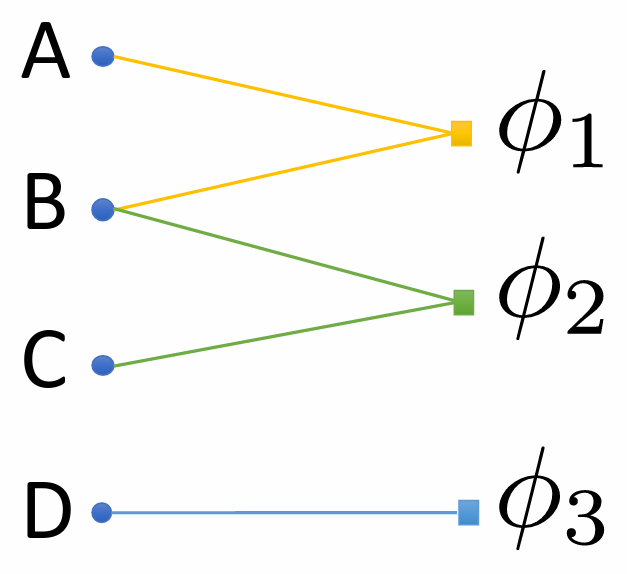
\includegraphics[scale=0.25]{images/factorgraph.PNG}
\end{figure}
\vspace{-0.5cm}
\[ P(A, B, C, D) = \frac{1}{Z} \ \phi_1(A, B) \ \phi_2(B, C) \ \phi_3(D) \]

\noindent
Note that $Z$ is the normalization constant.
Another graphical model is a \textbf{Markov network} (non-directed graph):

\begin{figure}[h]
    \centering
    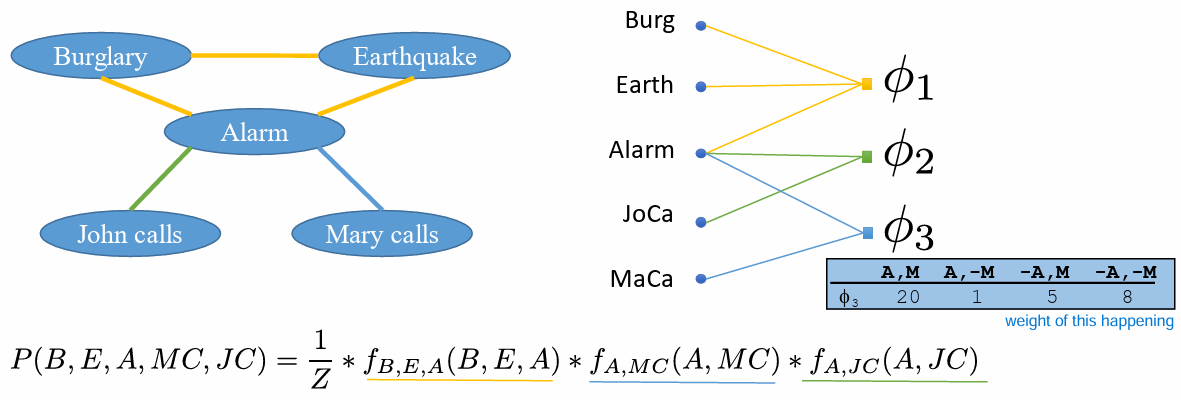
\includegraphics[scale=0.7]{images/markovnetwork.PNG}
\end{figure}

\noindent
Note that cliques are sets of nodes that are all connected to each other.
The directed version of a Markov network is a \textbf{Bayesian network}.
Bayesian networks use conditional probability tables, which are easier to interpret than factor graphs.
The final probability calculation is given by:

\[ P(X_1, ... , X_n) = \prod_{i} P(X_i | \text{parents}(X_i)) \]

\newpage
\begin{figure}[h]
    \centering
    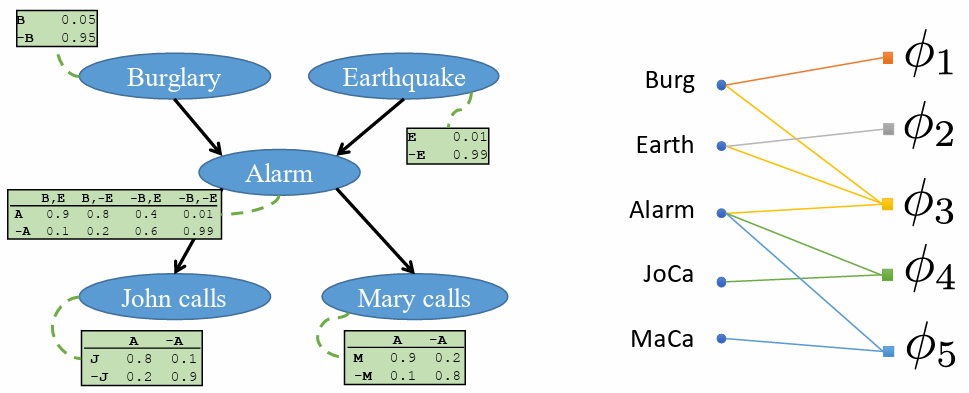
\includegraphics[scale=0.75]{images/bayesiannetwork.PNG}
\end{figure}

\noindent
While graphical models are a good middle way, they still have some problems to solve.
A big problem is that exact inference (e.g. $P(X = x)$) is NP-complete.
This is because we need to go over all possible combinations of variables, even those unobserved.

\noindent
\\
One way to do exact inference is to use \textbf{variable elimination}.
This is a dynamic programming algorithm that eliminates variables from the graph, until only the query variable is left.
The variable elimination algorithm works as follows, for each variable $X_i$:
\begin{enumerate}
    \item Multiply all factors $\phi_i$ that mention $X_i$.
    \item Marginalize out $X_i$ to obtain a new factor $\tau$.
    \item Replace all factors $\phi_i$ that mention $X_i$ with $\tau$.
\end{enumerate}

\subsection{Logic and Probability}
The current state of the art in expert systems focuses on combining the strengths of logic and probability.
This combination is mainly done through \textbf{probabilistic predicates}, for example:
\[ p: q(t_1, ... , t_n) \]

\noindent
Here all ground predicates $q(t_1, ... , t_n)$ are true with probability $p$.
Logical rules are applied the same way as in classical logic.
Here is an example of a program written in ProbLog, that models a graph where some edges might be missing:

\begin{figure}[h!]
    \centering
    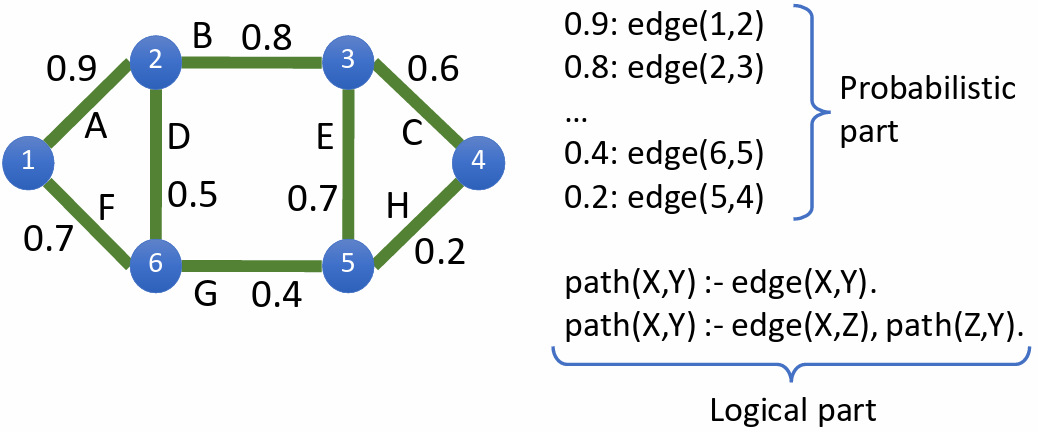
\includegraphics[scale=0.6]{images/problogexample.PNG}
\end{figure}

\newpage
\subsection{Machine Learning and Expert Systems}
Another state of the art in expert systems is the use of neural networks as logical predicates.
One example of this is giving a system two pictures of handwritten numbers (e.g. 3 and 5), and only telling the system the sum of the numbers (e.g. 8).

\noindent
\\
Historically, all expert systems used to be strictly rule-based.
Recently however, the field has shifted towards the inclusion of machine learning more and more.
A big use case of machine learning in expert systems is to keep the rule base up-to-date without expert input.
Some machine learning techniques like relational learning can even be used to learn first-order logic rules of concepts.
In some cases machine learning has replaced the rule base completely, most notably in the field of medical imaging.

\noindent
\\
In conclusion, expert systems have the following advantages:

\begin{itemize}
    \item Consistency (same input, same output).
    \item Memory (can store a lot of information).
    \item Logic (no biased decisions).
    \item Infinitely reproducible (does not get tired).
\end{itemize}

\noindent
However, expert systems also have the following disadvantages:

\begin{itemize}
    \item No common sense (cannot reason about the world).
    \item No creativity (cannot come up with new ideas).
    \item Frequent maintenance (rules need to be updated).
    \item Not adaptable by itself (no response to changing conditions).
\end{itemize}

%
% Topic 4 - Evolutionary Algorithms
%
\newpage
\section{Evolutionary Algorithms}
\textbf{Evolutionary computation} is a way to solve an optimization problem using a population of \textbf{candidate solutions} and the dynamics of \textbf{genetic evolution}.
These algorithms fall in a special category called \textbf{any-time algorithms}, meaning that you can let these algorithms run forever and just take a solution from it when you need it.
Evolutionary algorithms are also well known iterative processes, and rely heavily on stochasticity.

\subsection{Steps of an Evolutionary Algorithm}
Generally speaking, an evolutionary algorithm always follows the same steps:

\begin{enumerate}
    \item Construct an initial population.
    \item Select individuals for reproduction.
    \item Generate a new population from the reproduction pool.
\end{enumerate}

\noindent
Steps 2 and 3 are repeated until a stopping criterion is met.

\subsubsection{Population}
The initial population often consists of a randomly generated set of possible solutions.
These are usually low quality, but they can be seeded with domain knowledge for faster convergence.
The most important thing about the initial population is that it needs to be \textbf{large} and \textbf{diverse}.
The initial population acts as the basis of future solutions.

\noindent
\\
A \textbf{genotype} is the representation of a solution in the population.
A common example of a genotype is a bit string, but many data structures are possible as long as it can perform the necessary operations.
The actual solution that a genotype encodes is called the \textbf{phenotype}.
The most important difference between the two is that the phenotype can actually be evaluated for performance.

\subsubsection{Selection}
The selection criterion for an evolutionary algorithm is called the \textbf{fitness function}.
This is also the criterion that the algorithm tries to optimize.

\noindent
\\
The complexity of the selection procedure often determines the complexity of the whole algorithm.
This also limits the population size and the number of generations that can be computed.
One way to speed up the selection process is to use \textbf{sampling} (performing selection on a subset of the population, then generalizing).

\noindent
\\
Fitness-based selection is used to steer both the probability of survival for an individual, and the probability of inclusion in the reproduction pool.
This selection can be done using multiple methods, for example \textbf{roulette wheel selection} and \textbf{tournament selection}.

\newpage
\noindent
\textbf{Roulette wheel selection} is a method where the probability of an individual being selected is proportional to its fitness.

\begin{figure}[h]
    \centering
    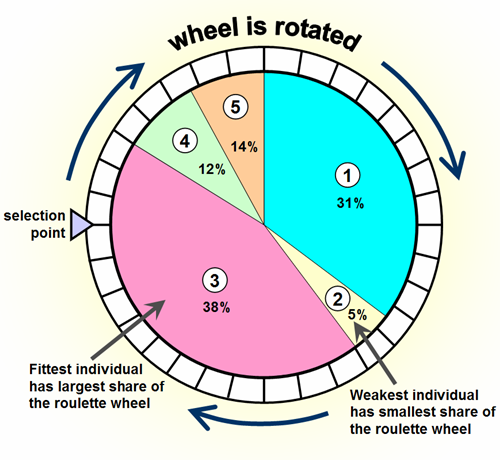
\includegraphics[scale=0.5]{images/roulettewheel.png}
\end{figure}

\noindent
The probability of being selected is often given by:
\[ p_i = \frac{f_i}{\sum_j f_j} \]

\noindent
Another way to calculate the probability of being selected is using the \textbf{Boltzmann distribution}:
\[ p_i = \frac{e^{f_i/T}}{\sum_j e^{f_j/T}} \]

\noindent
This equation features a temperature parameter $T$, which allows for tuning of the selection.
High values of $T$ lead to more random selection, while low values of $T$ lead to more deterministic selection based on fitness.

\noindent
\\
\textbf{Tournament selection} is another popular selection method.
The idea is to hold several limited-size tournaments and to select the winner of each tournament for the reproduction pool.
Smaller tournaments reduce the selection pressure, increasing the diversity of the population, but also leading to slower convergence.

\noindent
\\
Similarly to roulette wheel selection, tournament selection can also be tuned using some parameters.
The most important parameter is the tournament size $k$, which determines both how many individuals are in the tournament, and how many individuals are selected for the reproduction pool.
A different way to increase diversity without reducing selection pressure is to use \textbf{stochastic tournament outcomes}.
This means that the $i$'th best individual is selected with probability:
\[ p_i = p \left( 1 - p \right)^{i - 1} \]

\newpage
\subsubsection{Reproduction}
The idea of reproduction is to create a new population from the reproduction pool.
This can be done using a variety of operations, but the most common are \textbf{crossover} and \textbf{mutation}.

\noindent
\\
\textbf{Crossover} is the process of combining two genotypes to create a new genotype.
The most common form of crossover is \textbf{single-point crossover}:

\begin{figure}[h]
    \centering
    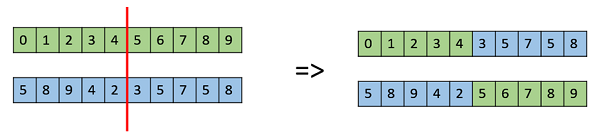
\includegraphics[scale=0.75]{images/singlepointcrossover.jpg}
\end{figure}

\noindent
Other forms of crossover include \textbf{multipoint crossover} (multiple points of crossover), \textbf{headless-chicken crossover} (crossover of a population member with a randomly generated genotype) and \textbf{uniform crossover}:

\begin{figure}[h]
    \centering
    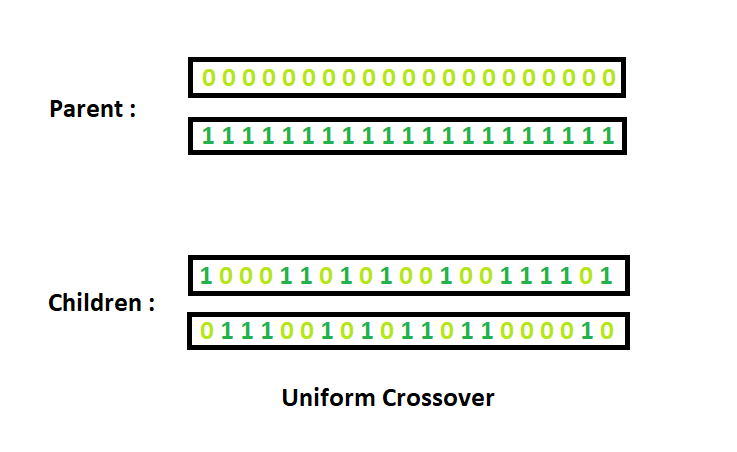
\includegraphics[scale=0.5]{images/unifromcrossover.png}
\end{figure}

\noindent
\textbf{Mutation} is the process of changing a genotype randomly.
This is done to maintain diversity in the population.
The key to mutation is to keep the mutation rate as low as possible, while still increasing population diversity.

\noindent
\\
The most common form of mutation is \textbf{bit-flip mutation}, where only a single bit in the genotype is flipped (or sometimes the whole genotype).
Another common form of mutation is \textbf{real-value mutation}, where a random value is added to the genotype (often some Gaussian noise).
There are many other forms of mutation, depending on the exact structure of the genotype.

\subsection{Schema Theory}
The rules of behavior for evolutionary algorithms are relatively simple.
However, the resulting dynamics are difficult to understand.
\textbf{Schema theory} offers some insight into why good solutions survive and get combined into even better solutions.

\noindent
\\
Consider the following binary genotypes: $0110$, $1110$, $1100$, $0100$.
All these instances belong to the schema *1*0, where * indicates positions where the exact value does not matter.

\newpage
\noindent
Consider fixed-length schemata of the form:
\[ s \in \{0, 1, \text{*}\}^n \]

\noindent
The \textbf{order} $o(s)$ is the number of fixed positions in $s$.
The \textbf{defining length} $d(s)$ is the longest distance between fixed positions in $s$.
We can use these definitions to reason about the disruptive properties of mutation and crossover.

\noindent
\\
The probability of a schema to survive mutation is given by:
\[ \left( 1 - p_m \right)^{o(s)} \]

\noindent
Where $p_m$ is the probability of mutation for a single bit.
We can deduce from this that schemata with a higher order have a lower probability of surviving mutation.

\noindent
\\
The probability of a schema to survive single-point crossover is given by:
\[ 1 - p_c \frac{d(s)}{n - 1} \]

\noindent
Where $p_c$ is the probability of crossover.
We can deduce from this that schemata with a higher defining length have a lower probability of surviving crossover.

\noindent
\\
Of those schemata with above average fitness, those with \textbf{low order} and \textbf{short defining length} are more likely to survive.
This is called the \textbf{schema theorem}.

\noindent
\\
If we generalize this to evolutionary algorithms, we can say that evolutionary algorithms work by identifying and combining \textbf{building blocks} that take the form of schemata with low order and short defining length.
This gives us some guidelines for designing genotypes:

\begin{itemize}
    \item Put related genes close to each other, so that they can form schemas with low description length.
    \item Make each gene as independent of other genes as possible.
    \item Give the crossover operator a low probability of destroying schemas.
\end{itemize}

\noindent
Since crossover and mutation can be destructive to good schemata, we are constantly at the risk of losing good solutions.
A possible solution to this is to use \textbf{elitism}, where the best $k$ solutions are always included in the next generation.

\subsection{Separable Natural Evolution Strategy}
If each gene is independent of other genes, then we can turn each gene into a probability distribution.
\textbf{Separable Natural Evolution Strategy} (SNES) is an evolutionary algorithm that maintains a Gaussian distribution $(\mu, \sigma)$ for each gene.
An individual from the population is generated by sampling each gene from its distribution.
SNES has no traditional selection and reproduction.
Instead, the means and standard deviations are updated using a weighted sum of the individuals (fit individuals have a larger say).
This can be seen as a gradient, moving into the direction of the fittest individuals.
Mutation is covered by resampling every generation.
This ensures diversity and prevents suboptimal convergence.

\newpage
\subsection{Problems with Evolutionary Algorithms}
A niche solution can draw a lot of the population towards a suboptimal solution.
If too many individuals become similar, crossover does not result in any more search.
Only mutation can get the population out of such a situation, but this is a slow process.
In general, evolutionary algorithms give no 'guarantee' about the quality of the solution that will be reached.

\noindent
\\
To avoid overpopulation of similar individuals, any group of sufficiently similar individuals (\textbf{nice radius}) can have a penalty added to their fitness evaluation.
Another solution is to actively monitor premature convergence, and simply replace parts of the population with randomly generated individuals.

\noindent
\\
A big problem for evolutionary algorithms is that they don't scale well with problem complexity.
The building block theory suggests that the full solution should be divisible into smaller, partial solutions.
However, for many intrinsically complex problems this is not the case.

\noindent
\\
Another difficulty for evolutionary algorithms is that they need a sufficient fitness function.
A fitness function must be able to separate partial solutions from non-solutions, with a sufficient spread in fitness values.
This means that evolutionary algorithms cannot solve problems with a binary fitness function (i.e. solved / non-solved).

\subsection{Neuro-Evolution}
Neuro-evolution is the use of evolutionary algorithms to train artificial neural networks.
In neuro-evolution the genotype can represent many things, for example:

\begin{itemize}
    \item Weight values.
    \item Number of processing units.
    \item Topology.
    \item Learning rate.
    \item Etc.
\end{itemize}

\noindent
To compute the fitness of a genotype, it is first translated into its corresponding phenotype (a neural network).
Each neural network is then evaluated on the actual task, and both the training and performance evaluation combined produce the fitness.

\noindent
\\
A neural network can either be \textbf{directly} or \textbf{indirectly} encoded as a genotype.
In a \textbf{direct encoding}, the genotype holds binary or real number representations of the weights, number of nodes, layers, etc.
In an \textbf{indirect encoding}, the genotype operates at a higher level of abstraction.

\noindent
\\
An example of an indirect encoding is compressing the weight matrix.
Weights in each dimension of the weight matrix can be treated as signals, and thus also be compressed.
This means that we can use wavelet-based compression to encode the weight matrix as a genotype.
This also (weakly) decouples the genotype size from the network complexity.

%
% Topic 5 - Agent Coordination
%
\newpage
\section{Agent Coordination}
Industry 4.0, also called the fourth industrial revolution, refers to the current trend of integrating digital technologies into manufacturing and industrial processes.
This includes the use of the Internet of Things (IoT), cloud computing, cognitive computing, as well as situated agents.
A common example of agents situated in an industrial environment are robots moving packages around a warehouse.
Having multiple agents operating in the same environment brings up a few challenges, most notably the challenge of \textbf{agent coordination}.

\subsection{Coordination Theory}
The concept of coordination has multiple definitions.
A few examples are:

\begin{itemize}
    \item Managing dependencies between activities (Malone '94).
    \item Special case of interaction in which agents are aware of their dependencies on other agents and adjust accordingly (Malone '91).
    \item Any decision that uses information concerning the existence, decisions or decision-making strategies of others (Stirling '94).
\end{itemize}

\noindent
The main components of coordination are as follows:

\begin{itemize}
    \item \textbf{Goals}: what are the agents trying to achieve?
    \item \textbf{Activities}: what tasks need to be performed to achieve the goals?
    \item \textbf{Actors}: who is responsible for performing the activities?
    \item \textbf{Interdependencies}: how do the activities of the actors relate to each other?
\end{itemize}

\noindent
Interdependencies are often considered the most important component of coordination.
Common Interdependencies include \textbf{prerequisites} (output of one activity is required for another), \textbf{shared resources} (some resources are required by multiple activities) and \textbf{simultaneity} (multiple activities must be performed at the same time).

\noindent
\\
A common question asked in agent coordination is why agents should coordinate at all.
After all, a central control system is often easier to implement.
The answer relates to the principle of \textbf{bounded rationality}.
This principle states that rationality is limited when individuals make decisions, and that, under these limitations, rational individuals will select a decision that is satisfactory, rather than optimal.
In addition to this, some modern systems are too complex to be controlled by a single entity.
This also relates back to \textbf{distributed intelligence}.

\subsection{Methods for Coordination}

\subsubsection{Client-Server}
In a client-server model, the client sends a request for operations to the server, who is responsible for the coordination of its clients.
The role of client or server can be dynamically played by agents.
Some agents can be both client and server at the same time, and some servers can be clients to other servers.
The pros of this model are that it is simple and easy to implement, while the downsides are that servers may become bottlenecks, there is a lack of failure tolerance, and the information used by servers may be out of date.

\newpage
\subsubsection{Task-Result Sharing}
The idea behind the task-result sharing model is that tasks get decomposed into subtasks, which are then distributed to agents.
The subsolutions to these subtasks are then combined to form the solution to the original task.
An example of task-result sharing is the \textit{MapReduce} algorithm, which is used to process large amounts of data in parallel:

\begin{figure}[h]
    \centering
    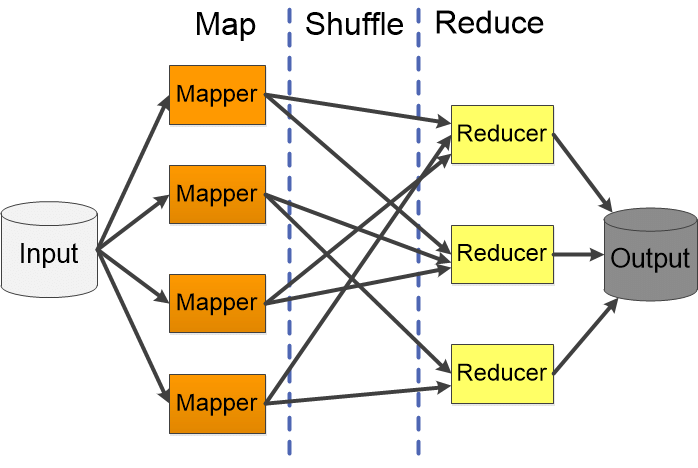
\includegraphics[scale=0.35]{images/mapreduce.png}
\end{figure}

\noindent
Subtasks can be related to each other in a variety of ways.
The most common subtask relations are:

\begin{figure}[h]
    \centering
    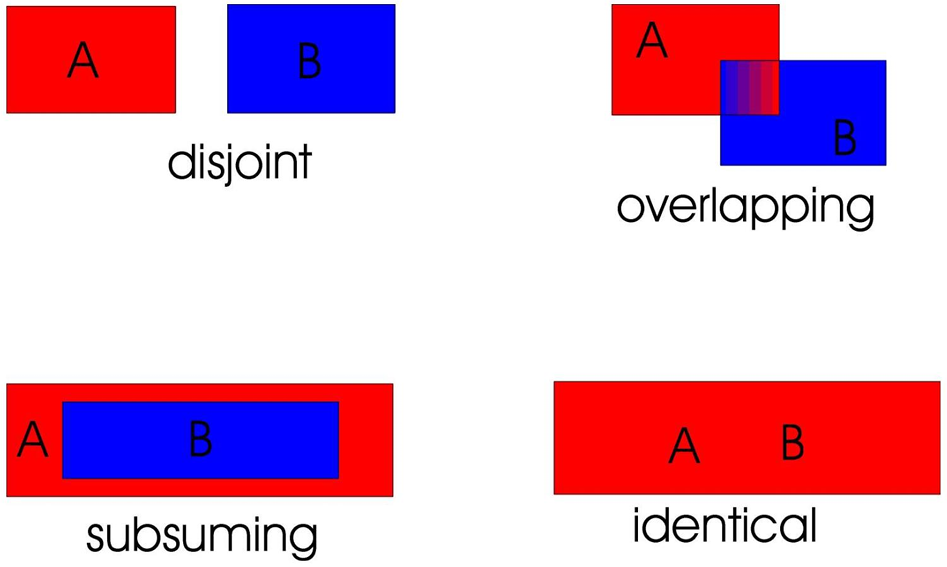
\includegraphics[scale=0.35]{images/subtaskrelations.PNG}
\end{figure}

\noindent
The potential advantages of task-result sharing are that each sub-problem can be solved with fewer knowledge and less resources.
In addition to this, the task-result sharing model is scalable, robust and uses parallelism in its core.

\noindent
\\
One of the key challenges involved in task-result sharing is that it is still unclear who is responsible for the coordination of the subtasks.
In addition to this, it is unclear what each entity needs to know, and how decomposed the tasks should be.
Finally, the task-result sharing model is very complex to implement.
Going more in-depth into the programming of all this could be a whole course on its own.

\subsubsection{Blackboard Model}
The core idea behind the blackboard model is that multiple agents read from and write to a shared memory space.
These read/write operations can be performed independently or in a coordinated way.
A key concept of the blackboard model is that all operations on the blackboard do not need to be traced back to a single entity.
All of this makes the blackboard model very suited for open, data- / event-driven applications, while supporting a variability in expertise as well as the incremental generation of solutions.

\newpage
\subsubsection{Contract Net Model}
The contract net model acts as a very simple negotiation protocol.
The idea is that we have a network of nodes (cooperating agents) acting as managers and contractors.
A \textbf{manager} announces a task to be done, and \textbf{contractors} respond with bids for the right to perform the task.
The contractor who bids the highest is awarded the task by the manager.
Similarly to the client-server model, the roles of manager and contractor can be dynamically played by agents throughout the process.

\noindent
\\
In general, the contract net model acts as a middle ground between the client-server model and the blackboard model.
The contract net model still faces the following design issues:

\begin{itemize}
    \item What tasks should be announced? When should an entity do a task instead of announcing it?
    \item Who should receive a specific announcement?
    \item Why should contractors bid for a task?
\end{itemize}

\subsubsection{Functionally Accurate Cooperation (FA/C)}
Functionally Accurate Cooperation (FA/C) is a guideline for cooperation when the individuals' local knowledge is incomplete or inconsistent.
Once this is noticed, agents should respond by exchanging \textbf{functionally correct information} (i.e. reasonable from a local point of view), and refining this into global correctness. 
For FA/C to work, all involved parties must be able to:

\begin{itemize}
    \item Measure and evaluate functional correctness.
    \item Detect inconsistencies between local and global knowledge.
    \item Revise and extend its local knowledge on the basis of newly obtained information.
\end{itemize}

\subsection{Advanced Methods for Coordination}
\subsubsection{Auctioning}
Auctioning is a method for coordination where agents bid for the right to perform a task (see: contract net model).
Many protocols for auctioning exist, some examples include:

\begin{itemize}
    \item \textbf{English Auction}: bidders are free to raise their bid, auction ends when no bidder is willing to raise anymore.
    \item \textbf{First-Price Sealed-Bid Auction}: each bidder submits one bid without knowing the others' bids, the highest bidder wins.
    \item \textbf{Vickrey Auction}: each bidder submits one bid without knowing the others' bids, the highest bidder wins, but pays the second-highest bid.
    \item \textbf{Dutch Auction}: auctioneer starts with a high price, and lowers it until a bidder accepts.
\end{itemize}

\noindent
Auctions can be characterized by the \textbf{valuation} of the goods and the \textbf{risk attitude} of the bidders:

\newpage
\begin{itemize}
    \item In a \textbf{private value auction} each bidders' value of the good is solely determined by their own preferences (e.g. an art auction).
    \item In a \textbf{common value auction} each bidders' value of the good is determined by the preferences of all bidders (e.g. an auction for a house).
    \item A \textbf{risk-averse bidder} is a bidder who would prefer to get the good, even if they have to pay more than their private valuation.
    \item A \textbf{risk-averse auctioneer} is an auctioneer who would prefer to sell the good, even if they could get more for it under different circumstances.
\end{itemize}

\noindent
An auction in between a private value auction and a common value auction is called a \textbf{correlated value auction}, while a bidder or auctioneer in between risk-averse and risk-seeking is called \textbf{risk-neutral}.

\noindent
\\
In general, all 4 auction protocols described above produce the same expected revenue for the auctioneer in a private value auction with risk-neutral bidders.
Among risk-averse bidders, a Dutch or First-Price Sealed-Bid auction gives higher revenue to the auctioneer, while risk-averse auctioneers can get a higher expected revenue through a Vickrey or English auction.

\subsubsection{Voting Systems}
Whenever there are multiple options to choose from, a voting system can be used to select option that best represents the preferences of the voters.
The two most common voting systems are \textbf{plurality voting} and \textbf{binary voting}.

\noindent
\\
In a \textbf{plurality voting} system, each voter can only vote for one option.
At the end of the voting, the option with the highest number of votes wins.
One of the biggest downsides of plurality voting is that it can lead to \textbf{strategic voting}, where voters vote for an option that is not their favorite, but has a higher chance of winning.
Another downside is that an \textbf{irrelevant alternative} can split the majority vote, leading to an overall less preferred option winning.

\noindent
\\
In a \textbf{binary voting} system, options are voted on in pairs.
This leads to an elimination bracket where the least preferred option is eliminated in each round.
Whichever option is left at the end of the bracket wins.
The biggest downside of binary voting is that the \textbf{agenda} (i.e. the order of the pairings), can have a big influence on the outcome.

\noindent
\\
A more preferred voting system is the \textbf{Borda protocol}.
In the Borda protocol, each voter ranks all options from most to least preferred.
If there are $n$ options, then the most preferred option gets $n$ points, the second most preferred option gets $n - 1$ points, and so on.
The option with the most points at the end wins.
Although the Borda protocol is less susceptible to strategic voting, it is still susceptible to irrelevant alternatives (although less than other options).

\subsubsection{Negotiation}
\textbf{Negotiation} is the exchange of information between two or more parties in multiple rounds, for the purpose of coming to an agreement.
A negotiation can be characterized by the \textbf{negotiation language}, \textbf{negotiation process} and \textbf{negotiation decision}, but this is beyond the scope of this course.

\newpage
\subsubsection{Joint Planning}
\textbf{Joint planning} is the notion of combining the individual plans of multiple agents into a single, coordinated plan.
The key design questions for joint planning are:

\begin{itemize}
    \item What exactly means a coordinated plan in this environment?
    \item How can parties detect "(un)coordinatedness"?
    \item How to jointly generated coordinated plans?
\end{itemize}

\noindent
A classical method for joint planning is \textbf{Partial Global Planning (PGP)}.
This is a general coordination schema, with no assumptions about sub-problems, expertise or resources.
It is essentially the joint planning version of FA/C.

\noindent
\\
The basic idea behind PCP is that each involved party can represent and reason about the actions and interactions of other parties, and how they affect local activity.
A \textbf{partial global plan} is a plan that specifies how different parts of a whole plan achieve a common goal.
A partial global plan consists of the following components:

\begin{enumerate}
    \item \textbf{Objective}: the reason why the PGP exists, including its goal.
    \item \textbf{Plan-Activity Map}: what the parties are doing, and how it contributes to the objective (including costs and expected results).
    \item \textbf{Solution-Construction Graph}: information about how the parties should interact, what results should be exchanged and when to exchange them.
\end{enumerate}

\noindent
The key limitations of PGP are that local actions may be executed without a joint agreement, and that the planned coordination is based on a very simple layer of abstraction.

\subsubsection{Commitments and Conventions}
A \textbf{commitment} is a promise to perform an action, and is often used as an abstraction to model the obligations of agents.
Commitments have the following operations:

\begin{itemize}
    \item \textbf{Create}: initiate a new commitment.
    \item \textbf{Discharge}: successfully fulfill a commitment.
    \item \textbf{Cancel}: revoking a commitment (failure case).
    \item \textbf{Release}: giving up a commitment (neutral case).
\end{itemize}

\noindent
To shift a commitment from one agent to another is called a \textbf{delegation} or an \textbf{assignment}, depending on if the other agent is a debtor or creditor of the commitment.

\noindent
\\
A \textbf{convention} is a description of circumstances under which an agent should (or is allowed to) reconsider its commitments.
It is important to find a balance between the flexibility of conventions and the stability of commitments.
A description of how to behave towards others when commitments alter (e.g. inform, offer alternatives, etc.) is called a \textbf{social convention}.

\noindent
\\
The \textbf{Centrality Hypothesis} states that all coordination mechanisms can ultimately be reduced to (joint) commitments and their associated (social) conventions:
\[ \text{coordination } = \text{ commitments } + \text{ conventions} \]

%
% Topic 6 - Reinforcement Learning
%
\newpage
\section{Reinforcement Learning}
Imagine you want to teach a robot how to juggle.
A classical, supervised learning approach would be to give the robot a dataset of juggling movements, and let it learn from that.
However, this approach has a few downsides.
Most notably, you need to hire a professional juggler to learn from.
In supervised learning, you need to know the solution to the problem you are trying to solve beforehand.
A better way to teach the robot how to juggle would be to just give it the balls and let it try for itself.
This is the core idea behind \textbf{reinforcement learning}.

\noindent
\\
An important note about reinforcement learning is that reinforcement learning is not a solution technique, but a learning setting.
You cannot say "I will use reinforcement learning to solve this problem", but you can say "This is a reinforcement learning problem".
Reinforcement learning suffers from the same issues as other machine learning techniques.
Additionally, reinforcement learning suffers from sparse rewards, non-observable environments (the \textbf{Markov assumption} (future is independent of past) is often violated) and non-stable environments (e.g. the presence of other agents).
Some people also believe that reinforcement learning is not a good learning model, as it needs to make a lot of mistakes to learn a new task.

\subsection{Problem Definition}
The goal of a reinforcement learning problem is to learn a \textbf{policy} that says what action to take in a given state.
The key elements of a reinforcement learning problem are that the agent should learn from interactions with the environment (not examples), the agent receives delayed rewards (not immediate feedback) and the agent should balance exploration and exploitation.
A single agent reinforcement learning problem can be defined as a \textbf{Markov Decision Process (MDP)}:

\begin{itemize}
    \item $S$: set of states.
    \item $A$: set of actions.
    \item $\delta: S \times A \rightarrow S$: transition function (often unknown).
    \item $r: S \times A \rightarrow \mathbb{R}$: reward function (often unknown).
    \item $\gamma$: discount factor (how much future rewards are worth).
\end{itemize}

\noindent
Given this Markov decision process, the goal of the agent is to find a policy $\pi: S \rightarrow A$ that maximizes the \textbf{value function}:
\[ V^\pi(s_t) = \sum_{i = 0}^{\infty} \gamma^i r_{t + 1} \]

\noindent
This represents the sum of all future rewards starting from state $s \in S$ at time $t$, assuming you choose all future actions according to policy $\pi$.
The discount factor $\gamma$ is defined as follows:
\[ r_t = \gamma r_{t + 1} \]

\noindent
The discount factor is used to balance immediate rewards against future rewards.
This does two things:

\begin{enumerate}
    \item By restricting $\gamma$ to $[0, 1)$, we ensure that $V^\pi(s_t)$ will be finite.
    \item By giving more value to immediate rewards, we put some time pressure on the agent (an agent with $\gamma = 1$ will be fine with taking a longer path to a better reward, rather than taking immediate rewards).
\end{enumerate}

\newpage
\subsubsection{Nondeterministic Environments}
In nondeterministic environments, performing the same action in the same state might lead to different outcomes.
We can model this using slightly different transition- and reward functions:

\begin{itemize}
    \item $P^a_{ss^\prime}: S \times A \times S \rightarrow [0, 1]$: transition function (where $s$ is the current state and $s^\prime$ is the follow-up state).
    \item $R^a_s: S \times A \rightarrow \mathbb{R}$: reward function.
\end{itemize}

\noindent
In the context of learning a policy, this is all fine as long as the probability distributions are \textbf{stationary} (i.e. they do not change during the learning process).
A useful tool for both a (non)deterministic environment is a \textbf{probabilistic policy}:
\[ \pi(a | s): S \times A \rightarrow [0, 1] \]

\noindent
This policy gives the probability of taking action $a$ in state $s$, and can be used to balance exploration and exploitation.

\subsection{Policy Iteration}
To get the value of a policy, we can use the \textbf{Bellman equation}, which can be deduced from the value function:
\[ V^\pi(s_t) = \sum_{i = 0}^{\infty} \gamma^i r_{t + 1} \quad \rightarrow \quad V(s) = r(s, \pi(s)) + \gamma V(\delta(s, \pi(s))) \]

\noindent
To realistically compute this, you can either look ahead until some time $T$ (\textbf{finite horizon}), or always look a fixed number of steps ahead (\textbf{receding horizon}).
For nondeterministic environments and policies, the Bellman equation can be modified as follows:
\[ V(s) = r(s, \pi(s)) + \gamma \sum_{s^\prime \in S} P_\delta(s, \pi(s), s^\prime)V(s^\prime), \ \text{for stochastic environments.} \]

\[ V(s) = \sum_{a \in A} P_\pi(a | s) \left[ r(s, a) + \gamma \sum_{s^\prime \in S} P_\delta(s, a, s^\prime)V(s^\prime) \right], \ \text{for stochastic policies.} \]

\noindent
This looks very complicated, but all it is doing is multiplying the value of the next state by the probability of reaching that state.
These equations are called the \textbf{value update rules}, and can be used to iteratively compute the value of a policy, called \textbf{policy iteration}:

\begin{algorithm}
    \caption{Policy Iteration}
    \begin{algorithmic}[1]
        \State Initialize $V_0$ arbitrarily.
        \State $t = 1$;
        \While{$(\text{bellman\_error} > \Delta)$}
            \For{$s \in S$}
                \State $V_t^\pi(s) = r(s, \pi(s)) + \gamma \sum_{s^\prime \in S} P_\delta(s, \pi(s), s^\prime)V_{t - 1}^\pi(s^\prime)$
            \EndFor
            \State $t = t + 1$;
        \EndWhile
    \end{algorithmic}
\end{algorithm}

\newpage
\noindent
In words, policy iteration starts by giving each state a random value (1).
Next, we start iteratively updating the value of each state using the value update rules (4, 5, 7).
One iteration of these lines is called a \textbf{full backup} (going through every state and updating its value).
This process is repeating until the \textbf{Bellman error} (maximum change in value during the previous full backup) is smaller than some threshold $\Delta$ (3).

\subsection{Actor-Critic}
Getting the value of a policy is nice, but what we really want is the policy that gives the highest value.
We can do this by letting our policy select the action that gives the highest value in each state (according to the policy iteration algorithm):
\[ \pi_t(s) = \argmax_a \left[ r(s, a) + \gamma \sum_{s^\prime \in S} P_\delta(s, a, s^\prime) V^{\pi_{t - 1}}(s^\prime) \right] \]

\noindent
If we replace our previous policy with this new policy, we can guarantee policy improvement between iterations:
\[ \forall s \in S : V^{\pi_t}(s) \geq V^{\pi_{t - 1}}(s) \]

\noindent
By combining this policy improvement with policy iteration to get the value of the policy, we get the \textbf{actor-critic} algorithm:

\begin{algorithm}
    \caption{Actor-Critic Policy Iteration}
    \begin{algorithmic}[1]
        \State Initialize $\pi_0$ and $V_0$ randomly.
        \State $t = 1$;
        \While{the values are still changing}
            \State Update the value of the states using the value update rules. \Comment{\textbf{Critic}}
            \State Update the policy using the policy improvement rule. \Comment{\textbf{Actor}}
            \State $t = t + 1$;
        \EndWhile
    \end{algorithmic}
\end{algorithm}

\noindent
Note that this algorithm is guaranteed to converge to the optimal policy.
You know you have an optimal policy when the policy does not change anymore between iterations.

\subsubsection{Value Iteration}
During normal policy iteration, it is common to do multiple full backups before updating the policy.
In practice this is quite inefficient, as not every state is relevant to the agent.
\textbf{Value iteration} is a variation of the policy iteration algorithm that performs fewer backups before updating the policy.
How many backups you do before updating the policy can be modified, but note that as long as you update the value of single state, you are still guaranteed to converge to the optimal policy.

\noindent
\\
A common implementation of value iteration is called \textbf{real time dynamic programming}, where you only update the value of the state that the agent is currently in:
\[ V(s) = \max_a \left[ r(s, a) + \gamma \sum_{s^\prime \in S} P_\delta(s, a, s^\prime) V(s^\prime) \right] \]

\newpage
\subsection{Model-Free Reinforcement Learning}
All these algorithms are nice, but they all require advanced knowledge of the reward function and the transition function.
In practice, these are often unknown.
In these cases, we simply let the agent learn from experience.
This is called \textbf{model-free reinforcement learning}.

\subsubsection{Monte-Carlo Estimation}
The idea behind \textbf{Monte-Carlo estimation} is to estimate the value of a state by averaging the rewards of all episodes that pass through that state.
This essentially comes down to updating a running average of the value of a state, with the following update rule:
\[ \tilde{V}(s) = \tilde{V}(s) + \alpha \left( V_{MC}(s) - \tilde{V}(s) \right) \]

\noindent
Where $\alpha$ is the learning rate, and $V_{MC}(s)$ is the value of the state as estimated by Monte-Carlo estimation.

\subsubsection{Bootstrapping}
In Monte-Carlo estimation, we wait until the end of an episode to update the value of a state.
In \textbf{bootstrapping}, we only perform a single step of the policy and calculate the \textbf{temporal difference error (TD-error)} of the previous state and the current state:
\[ \tilde{V}(s) = \tilde{V}(s) + \alpha \left( r + \gamma \tilde{V}(s^\prime) - \tilde{V}(s) \right) \]

\noindent
Where the part between brackets is the TD-error.
You can think of a temporal difference error as follows:
If you learn a monkey that they will receive a piece of banana if they press a button, and then give them a piece of banana without them pressing the button, they will experience a (positive) temporal difference error.
On the contrary, if they press the button and you don't give them a piece of banana, they will experience a (negative) temporal difference error.

\subsection{Q-Learning}
\textbf{Q-Learning} is a model-free reinforcement learning algorithm that learns the value of a state-action pair.
The Q-value of a state-action pair is defined as the expected return of taking action $a$ in state $s$:
\[ Q(s, a) = r(s, a) + \gamma \sum_{s^\prime \in S} P_\delta(s, a, s^\prime) V^{\pi_{t - 1}}(s^\prime) \]

\noindent
The Q-value of a state-action pair can be estimated by, after travelling through the state-action pair, following the policy and updating the Q-value based on the rewards encountered:
\[ Q^{\pi_t}(s, a) = r(s, a) + \sum_{i = 1}^N \gamma^i r(s_i, \pi_t(s_i)) = \sum_{i = 0} \gamma^i r_i \]

\noindent
We can then define our policy as the action that maximizes the Q-value of a state:
\[ \pi_t(s) = \argmax_a Q^{\pi_{t - 1}}(s, a) \]

\noindent
The combination of these two equations is called the \textbf{Q-learning algorithm}:

\newpage
\begin{algorithm}
    \caption{Q-Learning}
    \begin{algorithmic}[1]
        \State Initialize $Q$ arbitrarily.
        \State Start in state $s$.
        \While{true}
            \State Choose an action $a$.
            \State Execute $a$ and observe $r$ and $s^\prime$.
            \State $Q(s, a) = Q(s, a) + \alpha \left[ r + \gamma \max_{a^\prime} Q(s^\prime, a^\prime) - Q(s, a) \right]$
            \State $s = s^\prime$
        \EndWhile
    \end{algorithmic}
\end{algorithm}

\noindent
Q-learning is probably the most famous reinforcement learning algorithm our there.
It is a model-free algorithm, meaning that we do not need to know the reward function or the transition function, and it is guaranteed to converge to the optimal policy (as long as all state-action pairs are visited often enough!).
The learning rate $\alpha$ should be small enough to allow the agent to explore the environment.
For this reason, it is often set equal to $\frac{1}{\text{visits}(s, a)}$.

\subsubsection{Bucket Brigade Value Updating}
Consider the case where we can only get a reward at the end of an episode (e.g. after playing a game of chess).
When the agent arrives in this goal-state, it would only update the value of the state-action pair that led to the goal-state.
This is very inefficient, as the agent would not learn anything from the other state-action pairs.
\textbf{Bucket brigade value updating} aims to speed up this process by keeping track of which path was followed to reach the goal-state, and then updating these state-action pairs in reverse:
\[ Q(s, a) = r + \gamma Q(s^\prime, a^\prime) \]

\noindent
Where $Q(s, a)$ is the current Q-value, $r$ is the reward received in the current state (i.e. 0 except in the goal-state), and $Q(s^\prime, a^\prime)$ is the Q-value of the next state-action pair.

\subsubsection{Exploration vs. Exploitation}
A key issue in reinforcement learning is the balance between exploration and exploitation.
To learn a good policy, the whole environment should be explored.
To sample good values however, the agent should execute the best policy.
Our ultimate goal is to create a selection strategy that is \textbf{Greedy in the Limit with Infinite Exploration (GLIE)}.
This means that:

\begin{enumerate}
    \item Given infinite time, all state-action pairs are visited infinitely often.
    \item Given infinite time, the policy converges to a greedy policy.
\end{enumerate}

\noindent
There are multiple selection strategies that achieve this:

\begin{enumerate}
    \item \textbf{$\epsilon$-Greedy}: with probability $\epsilon$, the agent selects a random action, otherwise it selects the best action.
    This is GLIE if $\epsilon$ approaches 0 at a rate of $\frac{1}{t}$ (can be scaled with a learning rate).
    \item \textbf{Boltzmann Exploration}: choose an action with probability:
    \[ P(a | s) = \frac{e^{Q(s, a)/T}}{\sum_{a^\prime} e^{Q(s, a^\prime)/T}} \]
    Here $T$ plays a similar role as in simulated annealing.
    Note that a non-zero limit on $T$ allows for infinite exploration.
    Boltzmann exploration is GLIE if $T$ approaches 0 at a rate of $\frac{1}{\ln t}$.
\end{enumerate}

\newpage
\subsubsection{SARSA}
Imagine we have a robot that is tasked to walk from location A to location B.
The optimal path is to walk along the edge of a cliff, but there also is a longer path that has no risks involved.
If we make our robot learn the optimal policy, it will naturally walk along the edge of the cliff.
While walking along the edge of the cliff, the robot might feel the need to explore the environment, and as a result fall off the cliff.
This example illustrates that sometimes we have to discourage the agent from taking risks, and only sticking to situations it knows.

\noindent
\\
\textbf{SARSA} is a model-free reinforcement learning algorithm that functions similarly to Q-learning.
The key difference is that SARSA updates the Q-value of the current state-action pair based on the action that the agent actually took, rather than the best action it could've chosen.
In formula form, this comes down to simply removing the $\max_{a^\prime}$ from the Q-learning update rule:
\[ Q(s_t, a_t) = Q(s_t, a_t) + \alpha \left[ r_t + \gamma Q(s_{t + 1}, a_{t + 1}) - Q(s_t, a_t) \right] \]

\noindent
In the above example, the robot would learn that walking along the edge of the cliff is dangerous, and would learn to take the longer path instead.

\noindent
\\
A different way to look at the difference between Q-learning and SARSA is that Q-learning is an \textbf{off-policy} algorithm, while SARSA is an \textbf{on-policy} algorithm.
An off-policy algorithm learns the optimal policy values, as long as there is enough exploration.
An on-policy algorithm will learn the values of the policy it is following.
If you want an on-policy algorithm to learn the optimal policy, you will have to use a GLIE selection strategy.

\subsubsection{Function Approximation}
Q-learning is great, but it suffers from the curse of dimensionality.
The size of a Q-table is defined by the number of states times the number of actions, which can easily become very large.
Even if you could theoretically store all these values in memory, the amount of experience required to precisely estimate these values would be infeasible.

\noindent
\\
\textbf{Function approximation} is a straightforward solution to this problem.
The idea is to approximate the Q-values using a function, rather than storing them in a table.
By turning the state-action pairs into features $X$ and the Q-values into labels $y$, we can train a regression model to predict the Q-values (i.e. supervised learning).
Instead of a Q-table, we now have a Q-function:
\[ Q(s, a, \omega) \]

\noindent
Where $\omega$ is the set of weights of the model.
This is a great idea, but how do we train this model?
After all, we still cannot compute the Q-values for all state-action pairs.
There are a few possible estimates for the Q-values: 

\begin{enumerate}
    \item \textbf{Monte-Carlo Estimates}: unbiased but noisy. Converges to global optimum.
    \[ Q(s, a) = \sum \gamma^i r_i \]
    \item \textbf{SARSA Estimates}: biased (each parameter is initialized randomly, so will always be off by the same amount) but less noisy. Converges close to local optimum (but will never reach optimality).
    \[ Q(s_t, a_t) = r_t + \gamma Q(s_{t + 1}, a_{t + 1}) \]
    \item \textbf{Q-Learning Estimates}: unstable and biased. Not guaranteed to converge.
    \[ Q(s_t, a_t) = r_t + \gamma \max_a Q(s_{t + 1}, a)  \]
\end{enumerate}

\subsection{Policy Search}
Using values to learn a policy is great, but they are unstable under generalization.
Labels change during learning, and the samples are not independent of each other.
Moreover, learning values is not really the target of reinforcement learning.
Our end goal is to learn a policy (i.e. what to do in which situation), the values are just a way to represent the goal, but in some cases the value function will encode more than necessary (e.g. distance to goal, size of rewards, etc.).

\noindent
\\
It would be a lot easier if we could directly learn the policy, without any intermediate steps.
To do this, we first need something that can describe the policy performance for the entire environment, a \textbf{policy objective function}.

\subsubsection{Steady-State Distribution}
A Markov decision process is \textbf{ergodic} if it is:

\begin{enumerate}
    \item \textbf{Recurrent}: every state is visited infinitely often.
    \item \textbf{Aperiodic}: the time between visits to a state is not fixed.
\end{enumerate}

\noindent
If a Markov decision process is ergodic, then it has a \textbf{steady-state distribution} $d^\pi(s)$:
\begin{figure}[h]
    \centering
    \begin{minipage}{.5\textwidth}
      \centering
      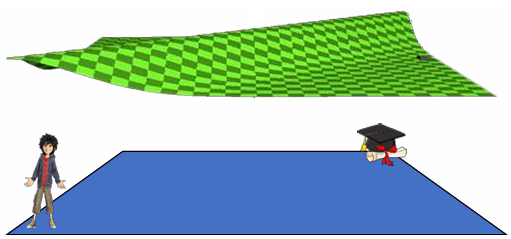
\includegraphics[scale=0.75]{images/mdp-ssd-1.PNG}
      \\An agent in an environment with a goal.
    \end{minipage}%
    \begin{minipage}{.5\textwidth}
      \centering
      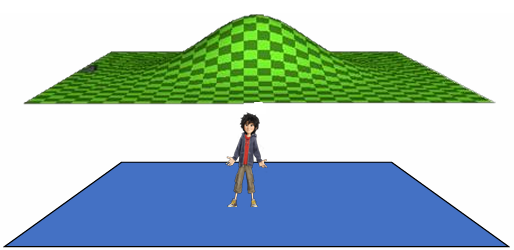
\includegraphics[scale=0.75]{images/mdp-ssd-2.PNG}
      \\An agent in an empty environment.
    \end{minipage}
\end{figure}

\noindent
The steady-state distribution is the probability of being in a state $s$ at any given time.
For example, if we put an agent in the middle of an empty environment, the steady-state distribution will look like a Gaussian curve.

\subsubsection{Policy Value}
The \textbf{policy value} is the expected value of following a policy $\pi$ in a given environment.
For episodic environments, the policy value is defined as the value of the start state, or the sum of the values of all possible starting states multiplied by the probability of starting in that state (in nondeterministic environments):
\[ \rho(\pi) = V^\pi(s_0) \quad \text{or} \quad \rho(\pi) = \sum_s P(s = s_0) V^\pi(s) \]

\newpage
\noindent
For continuous environments (i.e. the agent is never reset), the policy value is defined as the sum of the values of all states multiplied by the steady-state distribution:
\[ \rho(\pi) = \sum_s d^\pi(s) V^\pi(s) = \sum_{s, a} d^\pi(s) \pi(s, a) Q^\pi(s, a) \]

\noindent
If we represent the policy as a function with parameters $\theta$, then we can find the optimal policy by maximizing the policy value $\rho(\pi_\theta)$.
This can be optimized using any optimization algorithm, for example evolutionary algorithms:

\begin{algorithm}
    \caption{Evolutionary Policy Search}
    \begin{algorithmic}[1]
        \State Initialize a random population of candidate policies $<\theta_1, \theta_2, ... , \theta_n>$.
        \While{not converged}
            \State Evaluate each policy by letting an agent run for a time $T$. \Comment{Fitness = $\sum_{i = 0}^T \gamma^i r_i$}
            \State Combine the best policies to create a new population.
        \EndWhile
    \end{algorithmic}
\end{algorithm}

\subsubsection{Policy Gradient}
A more advanced optimization algorithm for policy search is \textbf{gradient ascent}.
Gradient ascent is usually more efficient than evolutionary algorithms, but it requires knowledge of the gradient of the policy value:
\[ \frac{\partial \rho(\pi_\theta)}{\partial \theta} \]

\noindent
Since the actual gradient is often unknown, we can approximate it by sampling the gradient at multiple points:
\[ \frac{\partial f(\theta)}{\partial \theta} = \frac{f(\theta + \epsilon) - f(\theta - \epsilon)}{2 \epsilon} \]

\noindent
Through some rewriting, we can find that, to compute the gradient of a policy, we only need the \textbf{score function}:
\[ \nabla_\theta \log(\pi_\theta(s, a)) \]

\noindent
We can estimate this score function by simply running around the environment and collecting data.
A famous algorithm that uses this idea is the \textbf{REINFORCE} algorithm:

\begin{algorithm}
    \caption{REINFORCE}
    \begin{algorithmic}[1]
        \State Initialize a random policy $\pi_\theta$.
        \While{not converged} \Comment{run around the environment}
            \For{$t = 1$ to $T$} \Comment{update weights every time step}
                \State $\theta = \theta + \alpha \nabla_\theta \log(\pi_\theta(s_t, a_t)) Q^{MC}(s_t, a_t)$ \Comment{gradient estimate $\cdot$ Monte-Carlo estimate}
            \EndFor
        \EndWhile
    \end{algorithmic}
\end{algorithm}

\noindent
In conclusion, direct policy search is a great way to learn a policy without having to remember what to do in every state.
This makes it very efficient in high-dimensional or continuous action spaces.
The potential downsides are that it can easily get stuck in local optima, and that it can be slow and suffer from a high variance.

%
% Topic 7 - Multi-Agent Reinforcement Learning
%
\newpage
\section{Multi-Agent Reinforcement Learning}
In the real world, agents often have to cooperate or compete with other agents.
Multi-agent systems are often very complex, highly dynamic and nondeterministic.
This makes multi-agent systems traditionally difficult to design, so maybe learning is a better approach.

\subsection{Cooperation vs. Competition}
When going from single-agent to multi-agent reinforcement learning, we have to reconsider some things:

\begin{itemize}
    \item What are the other agents doing? Where are they? What is their plan? The state space $S$ grows exponentially with the number of agents.
    \item All actions jointly influence state transitions and rewards. The action space $A$ grows exponentially with the number of agents.
    \item How to distribute the reward? Should the rewards be shared or only given to the agent that performed the final action?
\end{itemize}

\noindent
This last point is often referred to as the \textbf{credit assignment problem}.
In single-agent reinforcement learning, this refers to the problem of finding out which actions led to the reward.
In multi-agent reinforcement learning, we additionally have to consider which agents led to this reward.
When agents are cooperating with each other, various rewards are possible:

\begin{itemize}
    \item \textbf{Full System Reward}: a general reward, given to all agents.
    \item \textbf{Local Reward}: local feedback given to individual agents, could be useful for quicker learning.
    \item \textbf{Difference Reward}: give each agent feedback about its impact (rewards with vs without the agent's involvement).
\end{itemize}

\noindent
When agents are competing against each other, each agent usually has its own reward function.
In this scenario, the agents are trying to create a \textbf{best-response policy}.
A strategy is a best-response if it is optimal given the strategies of the other agents.
When all agents are playing a best-response strategy, we have a \textbf{Nash equilibrium} (i.e. nobody can improve by solely changing its policy).

\noindent
\\
Note that a Nash equilibrium is not necessarily the best outcome for all agents.
Jointly, the agents might be able to achieve a better outcome.
A \textbf{Pareto optimal} outcome is an outcome where no agent can improve without making another agent worse off.

\subsection{Normal Form Games}
Since action outcomes are jointly determined by all agents, a single agent's action does not influence the environment in a fixed manner.
This means that the best-response policy becomes a moving target, which violates the Markov assumption (essential for reinforcement learning).
We can solve this by modelling the environment as \textbf{normal form game}, for example:

\newpage
\begin{table}[h]
    \centering
    \begin{tabular}{c|c|c}
     & $b_0$ & $b_1$ \\ \hline
    $a_0$ & $r^{1a},r^{1b}$ & $r^{2a},r^{2b}$ \\ \hline
    $a_1$ & $r^{3a},r^{3b}$ & $r^{4a},r^{4b}$
    \end{tabular}
\end{table}

\noindent
We call this a \textbf{non-stationary / stateless environment}.
An advantage of stateless environments is that we do not need to accumulate awards over time, and can always simply look at the current state:
\[ Q(s, a) = r(s, a) \]

\noindent
A normal form game can have various properties, for example:

\begin{table}[h]
    \centering
    \subcaptionbox{Prisoner's Dilemma\\(\textbf{symmetric})}{
    \begin{tabular}{c|c|c}
     & $C$ & $D$ \\ \hline
    $C$ & $-3, -3$ & $0, -5$ \\ \hline
    $D$ & $-5, 0$ & $-1, -1$
    \end{tabular}}
    \hfill
    \subcaptionbox{Matching Pennies\\(\textbf{zero-sum})}{
    \begin{tabular}{c|c|c}
     & $H$ & $T$ \\ \hline
    $H$ & $1, -1$ & $-1, 1$ \\ \hline
    $T$ & $-1, 1$ & $1, -1$
    \end{tabular}}
    \hfill
    \subcaptionbox{Battle of the Sexes\\(\textbf{asymmetric})}{
    \begin{tabular}{c|c|c}
     & $B$ & $S$ \\ \hline
    $B$ & $2, 1$ & $0, 0$ \\ \hline
    $S$ & $0, 0$ & $1, 2$
    \end{tabular}}
\end{table}

\subsubsection{Q-Learning in Normal Form Games}
When tasked with making a reinforcement learning agent learn to play a normal form game, the first thing you might think of is to use Q-learning just like in a single-agent environment.
Interactions with other agents are considered noise in a stochastic environment.
This results in partial observability, which also means that the convergence of Q-learning is not guaranteed.
Still, Q-learning can still work in certain cases, for example in the battle of the sexes:

\begin{figure}[h]
    \centering
    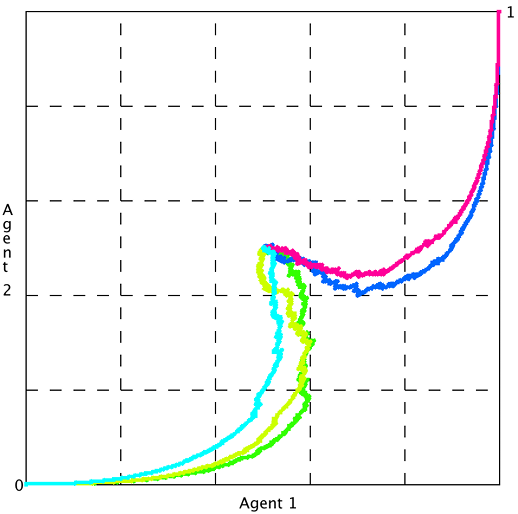
\includegraphics[scale=0.75]{images/battleofthesexes.PNG}
\end{figure}

\noindent
Here, the strategies of both agents converge to the two Nash equilibria in the game, $(0, 0)$ and $(1, 1)$.
This is an example where Q-learning works great, but this is not always the case:

\newpage
\begin{figure}[h]
    \centering
    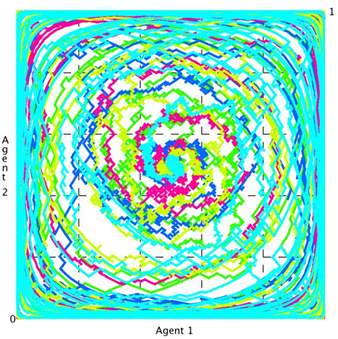
\includegraphics{images/matchingpennies.PNG}
\end{figure}

\noindent
Here you can see the results of Q-learning in the matching pennies game.
The agents are not converging to a Nash equilibrium, since this game's Nash equilibrium lies in mixed strategies.
Since Q-learning was not really a success, people have been looking for other algorithms that behave predictably (i.e. converge to an equilibrium), and behave rational (i.e. converge to a best-response).

\subsection{Learning Automata}
\textbf{Learning automata} is simply policy iteration for stateless environments.
Each agent has a vector with $|A|$ dimensions that stores the probability of taking each action:
\[ \pi_t = <\pi_t(a_1), \pi_t(a_2), ... , \pi_t(a_n)> \]

\noindent
Just like Q-learning, learning automata uses the immediate reward to update its action selection probabilities:
\[ \pi(a) = \pi(a) + \begin{cases}
    \alpha r_{t + 1}(1 - \pi(a)) - \beta(1 - r_{t + 1})\pi(a) & \text{if } a = a_t \\
    -\alpha r_{t + 1}\pi(a) + \beta(1 - r_{t + 1}) \left( \frac{1}{|A| - 1} - \pi(a) \right) & \text{otherwise}
\end{cases} \]

\noindent
Note that the reward has to be normalized to be between 0 and 1.
In the top case, the term $\alpha r_{t + 1}(1 - \pi(a))$ is called the \textbf{reward-term}.
If the agent receives a high reward after taking an unlikely action, the probability of taking that action will increase significantly.
The term $\beta(1 - r_{t + 1})\pi(a)$ in the top case is called the \textbf{penalty-term}.
If the agent receives a low reward after taking a likely action, the probability of taking that action will decrease significantly.
The bottom case balances the probabilities of all actions, ensuring that the sum of all probabilities is 1.

\subsubsection{Network of Learning Automata}
Learning automata was originally designed for stateless environments, but since its success it has also been successfully adapted to stateful environments.
In a \textbf{network of learning automata}, the agent uses a separate learning automata for each state.
When updating the probabilities, the agent uses the state-dependent reward to update the probabilities of the actions in that state:
\[ \bar{r} = \sum_{t = l + 1}^T \frac{r_t}{T - l} \]

\newpage
\noindent
Where $T$ is now, and $l$ is the last time the agent was in this state.

\subsubsection{Cross Learning}
$\alpha, \beta \in [0, 1]$ are called the reward- and penalty parameters.
If $\alpha = \beta$, then we have a \textbf{linear reward penalty}.
If $\beta = 0$ or $\beta = \epsilon$, then we have a \textbf{linear reward-inaction} or \textbf{linear reward-$\epsilon$-penalty}.
A special case of learning automata is \textbf{cross learning}, where $\alpha = 1$ and $\beta = 0$.
In this case the learning equation simplifies to:
\[ \pi(a) = \pi(a) + \begin{cases}
    r - r \pi(a) & \text{if } a = a_t \\
    -r \pi(a) & \text{otherwise}
\end{cases} \]

\noindent
Or, in vector notation:
\[ \pi(a) = (1 - r)\pi(a) + e_j r \]

\noindent
Where $e_j$ is a unit vector with a 1 at position $j$ (the action that was executed).
Note that once again, the reward has to be normalized to be between 0 and 1.

\noindent
\\
Cross learning originates from the field of psychology, and was actually invented earlier than learning automata.
The idea is that the change in probability for the action that was executed, $r - r \pi(a)$, is always positive.
This also increases the probability of actions that lead to bad rewards, but this actually models people's tendencies to repeat (bad) habits.
The only way to get out of a (bad) habit, is to execute a different action.

\subsection{Regret Minimization}
Similar to learning automata, \textbf{regret minimization} is another policy iteration algorithm for stateless environments.
The main difference is that regret minimization assumes hindsight knowledge of the best possible payoff, and uses that to calculate the loss $l$ for taking action $a$ instead of the best action $a^*$:
\[ l = r^* - r \]

\noindent
Regret minimization maintains a set of weights $w_j$, one for each action, and updates these weights according to the perceived loss:
\[ w_i = \begin{cases}
    w_i (1 - \alpha l) & \text{if } a_i = a_t \\
    w_i & \text{for all other } i
\end{cases} \]

\noindent
Note that the weights are not probabilities, so they do not have to sum to 1.
To get a legal policy, the weights can be normalized as follows:
\[ \pi(a_i) = \frac{w_i}{\sum_j w_j} \]

\subsection{Q-Learning with Multiple Agents}
The main difference between a stateless and a stateful environment is that an agent in a stateless environment gets immediate rewards, while an agent in a stateful environment gets a sum of delayed rewards.
However, if we use Q-values as immediate rewards, we can transform stateful environments into stateless environments.
This also means that, if we can compute Q-values for stateless environments, we can let algorithms designed for stateful environments learn in stateless environments.

\newpage
\subsubsection{Joint Action Learning}
\textbf{Joint action learning} aims to learn the Q-values for all joint actions in a stateless environment.
The main idea is that the agent keeps track off all action counts for all other agents $C^j_a$ (for agent $j$ and action $a$), and uses that to estimate the policy of the other agents:
\[ E[\pi^j(a)] = \frac{C^j_a}{\sum_{b \in A^j} C^j_b} \]

\noindent
The agent also learns the Q-values for all joint actions $a = <a^1, ... , a^m>$ (for $m$ agents), and uses these Q-values for its own policy by summing over all joint actions and multiplying them by the probability of them actually happening:
\[ E[V(a^i)] = \sum_{a^\prime \in A^{-i}} Q(a^\prime) \prod_{j \neq i} E[\pi^j(a^{\prime j})] \]

\noindent
Using joint action learning, it can become possible for agents to learn how to cooperate with each other.
The downsides are that it is very complex and computationally expensive, it assumes observing the actions of other agents is possible, and it assumes that the policy of other agents is static (not the case for learning-based agents).

\subsubsection{MiniMax-Q-Learning}
\textbf{MiniMax-Q-learning} is a model-free reinforcement learning algorithm that learns the Q-values for all joint actions in a stateful environment:

\begin{algorithm}
    \caption{MiniMax-Q-Learning}
    \begin{algorithmic}[1]
        \State Initialize $Q(s, a, o) = 1$ for all $s \in S, a \in A, o \in O$ \Comment{Q-values}
        \State Initialize $V(s) = 1$ for all $s \in S$ \Comment{Value function}
        \State Initialize $\pi(s, a) = \frac{1}{|A|}$ for all $s \in S, a \in A$ \Comment{Initial policy}
        \State
        \State Select action $a$ with probability $\pi(s, a)$, or a random action with probability $\epsilon$
        \State
        \State $Q(s, a, o) = (1 - \alpha)Q(s, a, o) + \alpha (r + \gamma V(s^\prime))$ \Comment{where $s^\prime$ is the new state}
        \State $\pi = \displaystyle\argmax_{\pi^\prime} \displaystyle\min_{o^\prime \in O} \displaystyle\sum_{a^\prime \in A} \pi^\prime(s, a^\prime) Q(s, a^\prime, o^\prime)$ \Comment{using linear programming}
        \State $V(s) = \displaystyle\min_{o^\prime \in O} \displaystyle\sum_{a^\prime \in A} \pi(s, a^\prime) Q(s, a^\prime, o^\prime)$
    \end{algorithmic}
\end{algorithm}

\noindent
Where $S$ is the set of states, $A$ is the set of actions and $O$ is the set of the opponent's actions.

\noindent
\\
MiniMax-Q-learning is designed for competitive zero-sum games, and makes fewer assumptions about the environment.
It converges to a safe strategy that maximizes the reward against the worst-case (i.e. best playing) opponent.
The only downsides are that it might be overkill for simple games, and that it cannot exploit exploitable opponents.

\subsubsection{Nash Q-Learning}
\textbf{Nash Q-learning} is a reinforcement learning algorithm designed to work with \textbf{general sum games} (games that do not need to sum to 1).

\newpage
\noindent
The main idea is that Nash Q-learning requires maintaining the \textbf{Nash Q-values} for both itself and its opponents.
The Nash Q-values are the expected sum of discounted rewards for all joint actions, given that all agents are playing a Nash equilibrium strategy:
\[ Q^*_i(s, <a_1, ... , a_m>) = r_i(s, <a_1, ... , a_m>) + \gamma \sum_{s^\prime} P_\delta(s, <a_1, ... , a_m>, s^\prime) V_i(s^\prime, <\pi^*_1, ... , \pi^*_m>) \]

\noindent
Where $<a_1, ... , a_m>$ are the joint actions of all agents and $<\pi^*_1, ... , \pi^*_m>$ are the Nash equilibrium policies of all agents.

\begin{algorithm}
    \caption{Nash Q-Learning}
    \begin{algorithmic}[1]
        \State $Q^0_j(s, <a_1, ... , a_m>) = 0$ for all $s \in S, <a_1, ... , a_m> \in A$
        \While{not converged}
            \State Choose action $a^t_i$, observe $<a^t_1, ... , a^t_m>, <r^t_1, ... , r^t_m>$ and $s^\prime$
            \State $Q^{t + 1}_j(s, <a_1, ... , a_m>) = (1 - \alpha_t)Q^t_j(s, <a_1, ... , a_m>) + \alpha_t (r^t_j + \gamma \text{Nash}Q^t_j(s^\prime))$
            \State $t = t + 1, s = s^\prime$
        \EndWhile
    \end{algorithmic}
\end{algorithm}

\noindent
Where $\text{Nash}Q^t_j(s^\prime)$ is the estimated value for agent $j$ from state $s^\prime$ onwards, assuming all agents play the Nash equilibrium as determined by the current Q-values.

\noindent
\\
Nash Q-learning is a very powerful and well-performing algorithm, but it also has some downsides.
Agents must be able to observe all rewards, not just their own.
Additionally, computing a Nash equilibrium for each agent at every step can be computationally expensive.

\noindent
\\
A similarly working algorithm is \textbf{friend-or-foe Q-learning}, which only works for zero-sum games.
The algorithm needs to know if it is dealing with a competitive or cooperative game, and uses different Q-values for each case.
The major advantage of friend-or-foe Q-learning is that it has a much stronger convergence guarantee than Nash Q-learning, to the point where it is basically guaranteed to converge.

\subsection{Policy Hill Climbing}
In \textbf{policy hill climbing}, we use two learning rates, $\alpha$ and $\delta$, to update the policy using a very simple gradient approximation:

\begin{algorithm}
    \caption{Policy Hill Climbing}
    \begin{algorithmic}[1]
        \State Initialize $Q(s, a) = 0, \pi(s, a) = \frac{1}{|A|}$ for all $s \in S, a \in A$
        \While{not converged}
            \State Select (with exploration) and execute action $a$, observe $r$ and $s^\prime$
            \State $Q(s, a) = (1 - \alpha)Q(s, a) + \alpha(r + \gamma \displaystyle\max_{a^\prime}Q(s^\prime, a^\prime))$
            \State $\pi(s, a) = \pi(s, a) + \begin{cases}
                \delta & \text{if } a = \displaystyle\argmax_{a^{\prime\prime}} Q(s, a^{\prime\prime}) \\
                \displaystyle\frac{-\delta}{|A| - 1} & \text{otherwise}
            \end{cases}$
        \EndWhile
    \end{algorithmic}
\end{algorithm}

\newpage
\subsubsection{Win or Learn Fast (WoLF)}
A popular variant of policy hill climbing is \textbf{Win or Learn Fast (WoLF)}.
The main difference is that WoLF uses two learning rates, $\delta_w$ (for when it's winning) and $\delta_l$ (for when it needs to learn fast).
It compares the expected value of the current policy to the average policy, and uses $\delta_w$ or $\delta_l$ depending on if it is currently doing better or worse:

\begin{figure}[h]
    \centering
    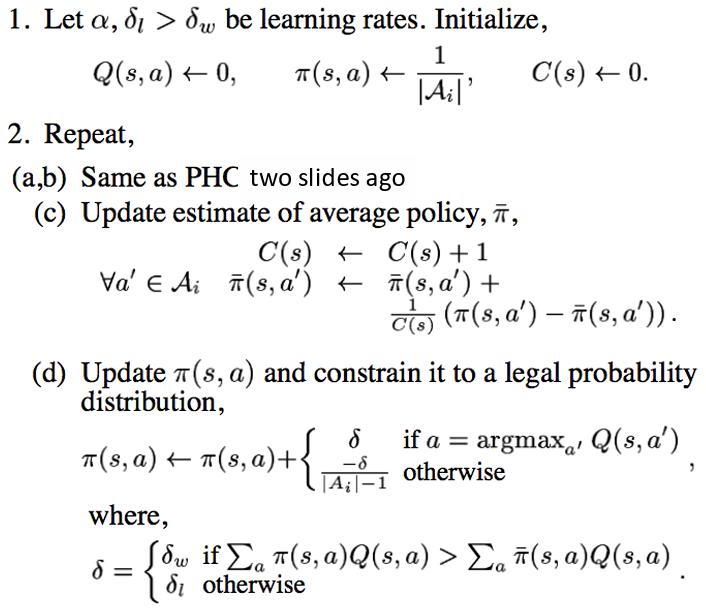
\includegraphics[scale=0.75]{images/WoLF.PNG}
\end{figure}

\noindent
Where $C(s)$ is the number of times state $s$ has been visited, and $\bar{\pi}(s, a)$ is the average selection probability of action $a$ in state $s$.

\end{document}
